\def\thudbabelopt{italian}
\documentclass[target=bach,aauheader=,style=]{thud}

\course{Informatica}
\title{Integrazione di Tecnologie Moderne per un CRM Efficiente: Un Caso Studio su Next.js}
\author{Alessandro Gerotto}
\supervisor{Prof.\ Vincenzo Riccio}
\tutor{Yannick Ponte}

\usepackage[a-1b]{pdfx}
\usepackage[pdfa]{hyperref}
\usepackage{multicol}
\usepackage{verbatim}
\usepackage{listings}
\usepackage{xcolor}
\usepackage{graphicx}
\usepackage{microtype}
\usepackage{geometry}
\usepackage{tocbibind}
\usepackage{array}
\usepackage{enumitem}
    \setlist{itemsep=.08em}
\usepackage{subcaption}
\usepackage{float}


\setlength{\intextsep}{30pt} 


\definecolor{backcolour}{rgb}{0.96,0.96,0.96}
\definecolor{codegray}{rgb}{0.5,0.5,0.5}

% Definizione del linguaggio JavaScript
\lstdefinelanguage{JavaScript}{
    backgroundcolor=\color{backcolour},
    basicstyle=\fontsize{10}{11}\ttfamily, 
    numberstyle=\color{codegray},
    keywords={break, case, catch, continue, debugger, default, delete, do, else, finally, 
              for, function, if, in, instanceof, new, return, switch, throw, try, typeof, 
              var, void, while, with, yield, const, let, async, await, import, export, 
              from, as, interface},
    keywordstyle=\color{blue}\bfseries,
    ndkeywords={class, boolean, implements, this, string, any, number, model, Project},
    ndkeywordstyle=\color{violet}\bfseries,
    sensitive=true,
    comment=[l]{//},
    morecomment=[s]{/*}{*/},
    commentstyle=\color{gray}\ttfamily,
    stringstyle=\color{gray}\ttfamily,
    morestring=[b]', morestring=[b]"
}

% Definizione del linguaggio React come estensione di JavaScript
\lstdefinelanguage{React}{
    language=JavaScript,
    alsoletter={<>=-},
    morekeywords={JSX, render, Component, useState, useEffect, useContext, 
                  useReducer, useRef, useCallback, useMemo, createContext, 
                  PropTypes, Fragment, className, =>},
    keywordstyle=\color{teal}\bfseries,
    morecomment=[s][\color{purple}]{<>}{</>},
    morestring=[b]`,
    sensitive=true
}

% Configurazione globale di lstlisting
\lstset{
    language=React,
    extendedchars=true,
    basicstyle=\footnotesize\ttfamily,
    showstringspaces=false,
    numbers=left,
    numberstyle=\footnotesize,
    numbersep=9pt,
    tabsize=2,
    breaklines=true,
    captionpos=b,
    aboveskip=10pt,
    belowskip=10pt
}




\begin{document}
\maketitle
%\begin{dedication}
%	Al mio cane,\par per avermi ascoltato mentre ripassavo le lezioni.
%\end{dedication}

%% Ringraziamenti (opzionali)
%\acknowledgements
%Sed vel lorem a arcu faucibus aliquet eu semper tortor. Aliquam dolor lacus, semper vitae ligula sed, blandit iaculis leo. Nam pharetra lobortis leo nec auctor. Pellentesque habitant morbi tristique senectus et netus et malesuada fames ac turpis egestas. Fusce ac risus pulvinar, congue eros non, interdum metus. Mauris tincidunt neque et aliquam imperdiet. Aenean ac tellus id nibh pellentesque pulvinar ut eu lacus. Proin tempor facilisis tortor, et hendrerit purus commodo laoreet. Quisque sed augue id ligula consectetur adipiscing. Vestibulum libero metus, lacinia ac vestibulum eu, varius non arcu. Nam et gravida velit.

%% Sommario (opzionale)
%\abstract
%Nunc ac dignissim ipsum, quis pulvinar elit. Mauris congue nec leo ornare lobortis. Nulla hendrerit pretium diam nec lobortis. Nullam aliquam laoreet nisl, sit amet facilisis lectus accumsan ut. Duis et elit hendrerit metus venenatis condimentum. Integer id eros molestie, interdum leo sit amet, aliquet metus. Integer fermentum tristique magna, vel luctus neque rhoncus vel. Ut hendrerit et quam et semper. Mauris egestas, odio sed aliquet luctus, magna orci euismod odio, vitae lacinia tellus tellus non lectus. Aliquam urna neque, porta et mattis aliquam, congue sit amet lorem. In ultrices augue sit amet ante vehicula, vitae rhoncus turpis auctor. Donec porta scelerisque eros, at mollis enim imperdiet ut. 

%% Indice
\tableofcontents

%% Lista delle tabelle (se presenti)
%\listoftables

%% Lista delle figure (se presenti)
%\listoffigures

%% Corpo principale del documento
\mainmatter

% Capitolo 1
\chapter{Introduzione}
\section{Introduzione generale}
Il presente lavoro di tesi si propone di analizzare il progetto di un software CRM (Customer Relationship Management) realizzato durante il periodo di tirocinio presso Archeido. L'obiettivo principale del progetto è stato quello di sviluppare una soluzione software efficace e innovativa, in grado di rispondere alle esigenze di gestione delle relazioni con i clienti. 

\noindent  Più nel dettaglio, lo scopo di questo progetto è sviluppare un CRM per gestire e monitorare i progetti in corso all'interno dell'azienda. Quando viene commissionato un nuovo progetto, questo viene registrato nella dashboard del CRM, dove è possibile tenere traccia delle tempistiche, dello stato di avanzamento e delle persone assegnate al progetto. Il sistema consente di monitorare l'intero ciclo di vita del progetto, dalla fase iniziale di pianificazione fino alla consegna finale, garantendo una gestione più efficiente delle risorse e una maggiore trasparenza nel processo operativo.

\noindent Per raggiungere questo obiettivo, è stato adottato un approccio di sviluppo basato su metodologie agili, che hanno consentito di adattare rapidamente le funzionalità del software alle necessità emergenti durante il processo di sviluppo.


\section{Struttura della tesi}

Nelle sezioni seguenti, si fornirà un'analisi dettagliata del prodotto software sviluppato, evidenziando le sue funzionalità principali, gli obiettivi prefissati e gli stakeholders coinvolti. Inoltre, verrà discusso il ciclo di vita adottato per il progetto, i problemi riscontrati e le valutazioni effettuate, nonché il percorso di formazione che ha affiancato il tirocinio. Successivamente, sarà fornita una panoramica delle tecnologie utilizzate e dei requisiti funzionali del sistema, accompagnata da diagrammi esplicativi per facilitare la comprensione del lavoro svolto. 

\noindent Infine, saranno discussi i metodi di testing impiegati, le aree che hanno ricevuto maggior attenzione e quelle che necessiterebbero di ulteriori verifiche. In prospettiva, saranno esplorate le opportunità di ampliamento del progetto, come l'integrazione di nuove funzionalità o l'ottimizzazione di quelle preesistenti. 

\section{L'importanza di un CRM}
Un sistema CRM (Customer Relationship Management) è un software progettato per supportare le aziende nella gestione delle relazioni con i clienti, fornendo una piattaforma centralizzata per raccogliere e organizzare informazioni sui clienti, le interazioni e le attività correlate. L'importanza di adottare un CRM è evidente in diversi contesti aziendali, poiché consente di migliorare la qualità delle relazioni con la clientela, ottimizzare i processi interni e supportare strategie di crescita orientate ai dati. 

\subsection{Vantaggi dell'uso di un CRM}
L'adozione di un CRM comporta una serie di vantaggi strategici e operativi per le aziende. Tra i principali vantaggi, possiamo identificare i seguenti:

\begin{itemize}
   \item \textbf{Centralizzazione e accessibilità dei dati}: un CRM permette di raccogliere tutte le informazioni sui clienti e sui progetti in un unico sistema accessibile ai vari dipartimenti aziendali. Ciò consente una maggiore coordinazione tra team (ad esempio vendite, marketing e assistenza).

   \item \textbf{Facilità di monitoraggio dei progetti}: un CRM permette di monitorare l'avanzamento di ogni progetto, assegnare e verificare compiti e tempistiche, e garantire che ogni fase venga portata a termine nei tempi previsti.

   \item \textbf{Miglioramento dell'efficienza operativa}: grazie alla possibilità di monitorare e automatizzare le attività, un CRM riduce il tempo necessario per gestire progetti e interazioni, abbassando i rischi di errore umano e velocizzando i processi decisionali.

   \item \textbf{Miglioramento della fidelizzazione e soddisfazione del cliente}: un CRM permette di gestire in modo personalizzato le interazioni con ogni cliente, aumentando la capacità di rispondere alle loro esigenze. Ciò contribuisce a costruire rapporti più duraturi e a migliorare il tasso di fidelizzazione.
\end{itemize}

\subsection{Alternative ai sistemi CRM}
Oltre ai software CRM progettati per la gestione delle relazioni con i clienti, le aziende possono considerare altre soluzioni per organizzare dati e processi. I fogli di calcolo, come Excel o Google Sheets, rappresentano una soluzione economica, flessibile e semplice, adatta a piccoli team o aziende in fase iniziale, ma limitata in scalabilità e automazione. I sistemi ERP, invece, offrono una gestione aziendale completa, che include funzionalità per contabilità, produzione e, in alcuni casi, CRM. Tuttavia, un ERP può risultare complesso e costoso, soprattutto se le aziende necessitano solo di strumenti per la gestione dei clienti. Infine, piattaforme di gestione progetti come Trello, Asana o Monday permettono di organizzare e monitorare le attività interne, ma non offrono le funzionalità avanzate di un CRM, come il tracciamento delle interazioni e l'analisi delle vendite.

\section{L'importanza di una soluzione cloud-native}
Adottare un CRM cloud-native offre accesso continuo ai dati da qualsiasi dispositivo, favorendo la collaborazione e il lavoro remoto. La scalabilità del cloud permette di adattare le risorse senza costi infrastrutturali, mentre la manutenzione e la sicurezza sono gestite dal fornitore, riducendo oneri per l'azienda. Inoltre, le soluzioni cloud-native si integrano facilmente con altre applicazioni, centralizzando i dati e automatizzando i processi, migliorando l'efficienza operativa dell'azienda.

\subsection{Conclusione}
La scelta di un sistema CRM è, in definitiva, determinata dalle esigenze aziendali specifiche e dal livello di complessità delle relazioni con i clienti che si intende gestire. Un CRM rappresenta un'opzione fondamentale per le aziende che desiderano migliorare l'organizzazione e la qualità delle proprie relazioni commerciali, con un vantaggio competitivo legato alla possibilità di creare esperienze cliente più personalizzate e gestire i progetti in modo più efficiente.

% Capitolo 2
\chapter{Background aziendale}
Questo capitolo fornisce un quadro dettagliato del contesto aziendale di Archeido. Vengono esplorate le specializzazioni di tale azienda nell'ingegneria del software e nella trasformazione digitale, ponendo l'accento sull'approccio cloud-native e sull'uso delle metodologie Agile.

\noindent Si presenterà il CRM come una soluzione centrale per il monitoraggio dei progetti, evidenziando le sue funzionalità principali e gli obiettivi strategici che intende perseguire. Inoltre, verranno identificati gli stakeholders coinvolti nel progetto e analizzato il ciclo di vita del software adottato, mettendo in luce l'importanza della flessibilità e dell'adattamento. 

\noindent Infine, saranno discussi i problemi affrontati e le decisioni critiche riguardanti le tecnologie utilizzate e il percorso di formazione intrapreso per garantire un'efficace implementazione del sistema.

\section{Archiedo}
Archeido \cite{archeido2024} è un'azienda specializzata nell'ingegneria del software, focalizzata sulla creazione e implementazione di soluzioni su architetture cloud-native e infrastrutture Cloud, utilizzando principalmente Amazon Web Services. La missione di Archeido è supportare le aziende durante il processo di trasformazione digitale e adozione del Cloud, offrendo un'assistenza sia tecnica che strategica con massima trasparenza. L'azienda adotta e si basa sulle metodologie Agile, garantendo un processo di sviluppo rapido, sicuro ed efficiente.

\section{Prodotto software}
Il software sviluppato e descritto in questa tesi è un CRM (Customer Relationship Management), progettato per servire come una dashboard centrale per il monitoraggio dei progetti attualmente in corso, come archivio completo di quelli già completati e come piattaforma di pianificazione per i progetti futuri.

\subsection{Funzionalità principali}
Il CRM offre una gestione completa dei progetti, facilitandone le operazioni di creazione, lettura, aggiornamento e cancellazione (CRUD). Inoltre, consente di monitorare gli utenti autorizzati ad accedere alla dashboard, i quali vengono creati tramite inviti generati e condivisi da un super amministratore. A ciascun utente viene assegnato un ruolo specifico, che definisce le regole di visibilità e le autorizzazioni di accesso alle informazioni presenti nella dashboard. Infine, il sistema consente di valutare le performances aziendali, fornendo dati e metriche utili per analizzare l'efficacia dei progetti e il rendimento complessivo del team.

\subsection{Obiettivi del software}
Il CRM ha come obiettivo principale valutare le stime concordate con i clienti, consentendo ai project manager di confrontare le previsioni iniziali stabilite insieme al cliente con i risultati effettivi ottenuti a progetto completato. In questo modo, è possibile identificare eventuali scostamenti e adottare misure correttive tempestive per garantire il successo del progetto. Il CRM sviluppato è dunque uno strumento di monitoraggio che fornisce un supporto strategico volto all'ottimizzazione delle relazioni con i clienti.

\subsection{Stakeholders}
Gli stakeholders di questo progetto includono:

\begin{itemize}
    \item I \textbf{Super Amministratori}, che gestiscono la creazione degli utenti, assegnano loro permessi e regole di visibilità e hanno accesso completo a tutte le sezioni del CRM. 
    \item I \textbf{Project Manager}, i quali ricevono un account per accedere alla dashboard e possono visualizzare solo i progetti a cui sono stati assegnati, limitando l'accesso ad alcune sezioni.
    \item I \textbf{Clienti}, le cui esigenze influenzano l'uso del CRM, poiché il sistema è progettato per rispondere meglio alle loro necessità.
\end{itemize}

\section{Ciclo di vita adottato}
Archeido adotta un ciclo di vita del software basato su metodologie agili, che consentono di gestire progetti in modo iterativo e incrementale. Lo sviluppo Agile si caratterizza per un approccio flessibile, orientato a fornire rapidamente software funzionante al cliente, garantendo aggiornamenti frequenti e miglioramenti continui. In questo contesto, le fasi di specifica, progettazione, sviluppo, validazione ed evoluzione si susseguono in un processo fluido e non fisso, caratterizzato da una continua negoziazione dei requisiti e raccolta di feedback.

\subsection{Plan-based vs Agile development}
La differenza tra Agile e lo sviluppo plan-based risiede principalmente nell'approccio alla gestione dei progetti e nella flessibilità di risposta ai cambiamenti. Nel modello plan-based, il processo di sviluppo è caratterizzato da una pianificazione dettagliata e rigida delle fasi del progetto, dove i requisiti vengono definiti all'inizio e rimangono relativamente statici per tutta la durata del ciclo di vita del progetto. Al contrario, le metodologie Agile, come Scrum e Kanban, pongono l'accento sulla collaborazione continua tra i membri del team e gli stakeholder, consentendo una maggiore adattabilità. I requisiti non sono definitivi e possono evolvere nel corso del progetto, permettendo al team di rispondere rapidamente alle esigenze emergenti.


\section{Formazione e Pair Programming}
Il periodo iniziale di questo tirocinio è stato dedicato alla formazione, durante la quale è stata approfondita la programmazione funzionale in JavaScript \cite{knowthen2024}, acquisendo le competenze necessarie per scrivere codice più efficiente, leggibile e mantenibile. In seguito, si è analizzato React \cite{udemyreactredux2024}, una libreria JavaScript sviluppata da Facebook per la creazione di interfacce utente interattive e componenti riutilizzabili, facilitando lo sviluppo di applicazioni web complesse. Infine, è stato esplorato Next.js, un framework che estende le capacità di React, permettendo il rendering lato server e facilitando la creazione di applicazioni web performanti.

\noindent Una parte fondamentale della formazione è stata lo sviluppo prevalentemente in modalità di \textbf{Pair Programming}, una pratica essenziale della metodologia \textbf{Extreme Programming (XP)}, che ha velocizzato e semplificato l'apprendimento grazie alla collaborazione diretta tra i membri del team. In questo approccio, due programmatori lavorano insieme su un singolo computer: uno scrive il codice (driver), mentre l'altro lo esamina e fornisce suggerimenti (observer o navigator), favorendo un continuo scambio di conoscenze e un confronto immediato sulle soluzioni.

\noindent L'adozione di XP ha migliorato significativamente la qualità del codice, grazie al feedback immediato e all'integrazione di pratiche agili come il \textbf{refactoring continuo} e la \textbf{revisione condivisa} del lavoro. Questo metodo ha permesso di mettere in pratica fin da subito le nozioni apprese nei corsi di JavaScript funzionale e React sopramenzionati, consentendo di affinare rapidamente le competenze tecniche e di adottare efficacemente pratiche di \textbf{clean code}, garantendo uno sviluppo più strutturato, di qualità e conforme alle best practices della scrittura del codice adottate in Archeido.

\section{Problemi e valutazioni}
Nelle prime fasi dello sviluppo, è stata condotta un'analisi approfondita per valutare quale tra le diverse tecnologie disponibili e librerie grafiche fosse più adatta per la realizzazione del progetto. Alla fine, si è deciso di utilizzare Next.js \cite{nextjs2024} e l'omonima libreria grafica NextUI \cite{nextui2024}. 

\noindent Un altro aspetto cruciale nella fase di sviluppo è stata la scelta tra l'utilizzo di JavaScript puro e l'adozione di TypeScript. Questa decisione ha comportato una valutazione approfondita dei vantaggi e degli svantaggi di entrambe le opzioni, considerando fattori come la tipizzazione statica, la manutenzione del codice e la scalabilità del progetto, approfonditi ulteriormente nelle sezioni seguenti.


% Capitolo 3
\chapter{Background tecnico}

\section{Introduzione}
In questo capitolo, verrà presentato il contesto tecnico del progetto, descrivendo nel dettaglio le tecnologie principali utilizzate: TypeScript, React, Next.js, AWS, Next UI e Tailwind CSS. 

\noindent Queste tecnologie rappresentano la base dell'architettura del sistema e sono state selezionate per le loro caratteristiche che consentono di sviluppare un CRM moderno, efficiente e altamente scalabile. Verranno analizzati i punti di forza di ciascuna tecnologia, con un focus su come ognuna di esse contribuisca alla creazione di un'interfaccia utente reattiva, di un'esperienza utente fluida e di una gestione robusta dei dati.

\section{JavaScript e TypeScript}
Nel contesto di questo progetto si è optato per l'utilizzo di \textbf{TypeScript} \cite{wikipedia:typescript}. Questa scelta è stata effettuata durante la fase iniziale di analisi dei requisiti e il motivo principale è stato che TypeScript presenta un \textbf{sistema di tipi statici} rispetto a JavaScript, che invece ne utilizza uno a tipizzazione dinamica. Questo significa che i tipi delle variabili, delle funzioni e delle proprietà vengono definiti al momento della compilazione e non cambiano durante l'esecuzione, permettendo di rilevare gli errori in fase di compilazione piuttosto che durante l'esecuzione. Tuttavia, il browser non può interpretare direttamente il codice TypeScript, il quale però è completamente compatibile con JavaScript. Infatti, prima di poter essere eseguito nel browser, il codice TypeScript deve essere convertito in JavaScript tramite un processo di compilazione. Questo processo è tipicamente gestito da strumenti come il TypeScript Compiler (tsc), Webpack, Babel e altri bundler che supportano TypeScript. Durante la compilazione, TypeScript verifica la correttezza dei tipi e successivamente trasforma il codice TypeScript in JavaScript, che può essere eseguito da qualsiasi browser. Un esempio pratico in cui JavaScript risulta problematico è il seguente: 

\begin{minipage}[t]{0.45\textwidth}
    \begin{lstlisting}[caption=Coercion in JavaScript]
const add = (a, b) => {
    return a + b;
}   
add("5", 10); // -> "510"
    \end{lstlisting}
\end{minipage}
\hfill
\begin{minipage}[t]{0.45\textwidth}
    \begin{lstlisting}[caption=Errore in TypeScript]
const add = (a: number, b: number) => {
    return a + b;
}  
add("5", 10); -> // Errore
    \end{lstlisting}
\end{minipage}

\noindent Qui viene dichiarata la funzione \texttt{add}, la quale esegue la somma degli argomenti \texttt{a} e \texttt{b} che riceve come input. In JavaScript, essendo un linguaggio a tipizzazione dinamica, non viene generato alcun errore perché viene applicata automaticamente la \textbf{coercion}, ovvero la conversione implicita di un tipo di dato in un altro per eseguire l'operazione richiesta. Nel caso di \texttt{add("5", 10)}, il numero \texttt{10} viene infatti convertito in una stringa \texttt{"10"} per consentire la concatenazione con \texttt{"5"}, producendo il risultato \texttt{"510"}. Questo accade in quanto l'operatore \texttt{+} in JavaScript somma i valori se entrambi sono numeri, ma effettua la concatenazione se almeno uno dei due è una stringa. Al contrario, in TypeScript la chiamata \texttt{add("5", 10)} provoca un errore di compilazione, poiché il linguaggio richiede esplicitamente che i parametri siano di tipo \texttt{number}. Per questo motivo, TypeScript offre un notevole vantaggio, poiché impedisce le conversioni implicite di tipi, che spesso sono causa di comportamenti imprevedibili.

\subsection{Le interfacce in TypeScript}
\noindent Un altro punto a favore viene evidenziato in contesti dove le applicazioni sono più complesse: TypeScript offre un'architettura di codice più chiara e strutturata, mettendo a disposizione le \textbf{interfacce}. Queste ultime fungono da \textit{blueprint}, definendo i tipi esplicitamente. Ad esempio, per poter creare un nuovo progetto all'interno del CRM, è necessario che esso segua una struttura definita. Attraverso l'uso delle interfacce, è possibile stabilire chiaramente quali proprietà e quali tipi di dati devono essere presenti, garantendo così la corretta integrazione e funzionamento all'interno del sistema. Durante l'analisi dei requisiti, è emerso che ogni progetto registrato deve includere i seguenti campi:

\begin{itemize}
    \item \textbf{ID univoco}: necessario per distinguere i diversi progetti.
    \item \textbf{Codice progetto}: può non essere univoco.
    \item \textbf{Nome del progetto}: la denominazione assegnata al progetto.
    \item \textbf{Data di inizio}: corrisponde alla data in cui il team inizia a lavorare attivamente sul progetto.
    \item \textbf{Data di fine}: corrisponde alla data prevista per la consegna finale del progetto.
    \item \textbf{Project Manager assegnati}: i responsabili del progetto.
    \item \textbf{Stato del progetto}: può essere uno tra i seguenti: \texttt{Not Started}, \texttt{In Progress} o \texttt{Completed}.
    
\end{itemize}

\noindent Questa specifica ha consentito di definire un'interfaccia \texttt{Project}, garantendo che chiunque la implementi debba rispettare lo schema riportato di seguito:

\begin{lstlisting}[language=React, caption=Interfaccia di progetto]
export interface Project {
    id: string;
    code: string;
    name: string;
    startdate: string | number;
    enddate: string | number;
    state: string;
    assignedTo: string;
}
\end{lstlisting}

\noindent Inizialmente, non era previsto che un progetto potesse essere assegnato a specifici Project Manager, quindi il sistema era configurato per consentire a tutti gli utenti di accedere a ogni progetto. Grazie a TypeScript, l'aggiornamento del sistema è stato notevolmente semplificato: modificando l'interfaccia, gli errori di compilazione sono stati segnalati automaticamente in tutte le parti del codice interessate, facilitando l'individuazione delle sezioni da aggiornare. Questo ha reso il processo di adeguamento più rapido e preciso, assicurando al contempo la qualità del software.

\begin{figure}[H]
    \centering
    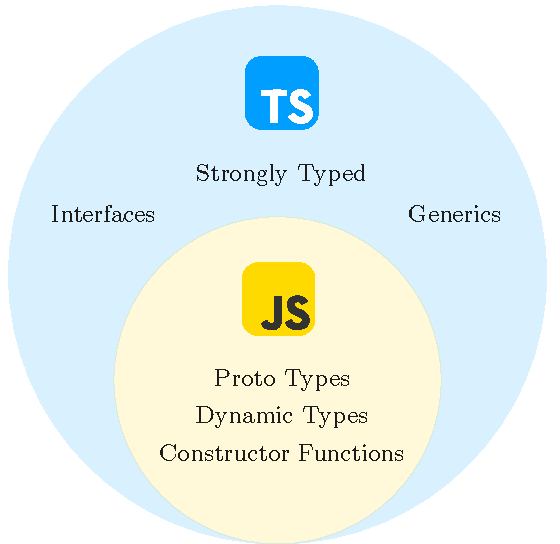
\includegraphics[width=0.4\textwidth]{img/typescript_and_javascript.pdf} 
    \caption{TypeScript e JavaScript}
\end{figure}

\section{React}
React è una libreria JavaScript per la creazione di interfacce utente reattive e componenti riutilizzabili. React consente di costruire interfacce utente utilizzando i cosidetti \textbf{componenti} sfruttando \textbf{JSX} (o \textbf{TSX} nel caso di TypeScript), una sintassi di estensione per JavaScript che permette di scrivere codice che combina quest'ultimo con HTML, in un formato che è più leggibile e comprensibile. Nell'esempio sotto riportato, il componente \texttt{Greeting} viene inizializzato usando JavaScript, ma restituisce un codice HTML:

\begin{lstlisting}[language=React, caption=Esempio di codice React]
const name = 'Alice';   
const Greeting = () => {
    return (
        <h1>
            Hello, {name}!
        </h1>
    )
} 
\end{lstlisting}

\subsection{I componenti}
Un componente React è una funzione JavaScript che rappresenta una parte riutilizzabile e autonoma di un'interfaccia utente in un'applicazione React. I componenti permettono di scomporre l'interfaccia in parti più piccole e gestibili, promuovendo la leggibilità, la manutenzione e il riuso del codice. Questo approccio basato sui componenti e sulla continua estrazione del codice in componenti più semplici garantisce diversi vantaggi:

\begin{itemize}
    \item \textbf{Riuso}: un componente può essere utilizzato in diverse parti dell'applicazione, riducendo la duplicazione del codice.
    \item \textbf{Isolamento}: ogni componente ha il proprio stato e le proprie proprietà, rendendo il singolo componente utilizzabile e testabile in ambienti isolati, rimuovendo le dipendenze da quanto appare al suo esterno.
    \item \textbf{Composizione di componenti}: una volta sviluppati diversi componenti, React consente di comporli insieme. Ad esempio, un componente \texttt{Card} potrebbe contenerne a sua volta tre più semplici: un'immagine, un titolo e un pulsante. Tale \texttt{Card} potrebbe venire poi usata molteplici volte all'interno di un componente più complesso, come un \texttt{Carousel}.
\end{itemize}

\subsection{Le \textit{props}}
Le props permettono a un componente genitore di fornire informazioni immutabili a un componente figlio, rendendo quest'ultimo più dinamico e flessibile.

\begin{minipage}[t]{0.45\textwidth}
    \begin{lstlisting}[caption=Componente padre]
import React from 'react';
import Greeting from './Greeting';

const App = () => {
    return (
        <div>
            <Greeting name= "Alice" />
            <Greeting name= "Bob" />
        </div>
    );
};  
    \end{lstlisting}
\end{minipage}
\hfill
\begin{minipage}[t]{0.45\textwidth}
    \begin{lstlisting}[caption=Componente figlio]
import React from 'react';

const Greeting = ({ name }) => {
    return (
        <h1>
            Hello, {name}!
        </h1>
    );
};

export default Greeting;
    \end{lstlisting}
\end{minipage}

\noindent In questo esempio, il componente \texttt{Greeting} (sulla destra) è una funzione che accetta la prop \texttt{name} e restituisce il testo  ``Hello," seguito dal valore di tale prop, ottenuta dal componente padre. 

\noindent Per esempio, quando viene passato ``Alice" come valore, come accade in \texttt{<Greeting name="Alice" />}, il risultato renderizzato sarà un'intestazione \texttt{h1} che riporta ``Hello, Alice!", mentre se viene passato ``Bob" (attraverso \texttt{<Greeting name="Bob" />}), verrà stampato ``Hello, Bob!".

\subsection{Gli hook}
Gli hook sono una caratteristica di React introdotta con la versione 16.8 che consente di utilizzare lo stato e altre funzionalità di React nei componenti funzionali, senza la necessità di convertire il componente in una classe. Gli hook forniscono un modo per gestire lo stato locale, eseguire effetti collaterali, e utilizzare contesti, tra le altre operazioni, rendendo il codice più pulito e riutilizzabile. 

\noindent Gli hook più comuni includono \texttt{useState}, che permette di mantenere e modificare lo stato locale all'interno di un componente, e \texttt{useEffect}, che consente di gestire effetti collaterali, come il caricamento di dati o la registrazione di eventi. Più nel dettaglio, \texttt{useState} restituisce un array composto da due elementi: il valore attuale dello stato (\texttt{selectedProject}) e una funzione per aggiornare tale valore (\texttt{setSelectedProject}). \texttt{useState} accetta un argomento, il quale rappresenta lo stato iniziale.

\begin{center}
\texttt{const [selectedProject, setSelectedProject] = useState<Project>({})}
\end{center}

\noindent \texttt{useEffect} invece, è un hook di React utilizzato per gestire \textbf{effetti collaterali} all'interno di un componente, come operazioni di recupero dati, manipolazione del DOM o registrazione di eventi. Accetta due argomenti: 

\begin{itemize}
    \item Una \textbf{funzione} che contiene il codice da eseguire (\texttt{() => {...}});
    \item Un \textbf{array} di dipendenze che specifica i valori da monitorare (\texttt{[...]}). Quando una di queste dipendenze subisce una modifica, il corpo di \texttt{useEffect} viene eseguito. Tale esecuzione spesso genera effetti collaterali, con conseguente cambiamento di stato. Quando ciò accade, si verifica un rendering aggiornato del componente. Se, come in questo caso, il secondo parametro è un array vuoto, la funzione passata come primo argomento all'hook verrà eseguita soltanto la prima volta.
\end{itemize}

\noindent Un esempio d'uso dei due hook sopracitati è il seguente, in cui si definisce una funzione chiamata \texttt{foo}. All'interno di questa funzione, viene utilizzato l'hook \texttt{useState} per creare una variabile di stato denominata \texttt{selectedProject} e la relativa funzione di aggiornamento \texttt{setSelectedProject}. L'inizializzazione di \texttt{selectedProject} è impostata su un oggetto vuoto, indicando che inizialmente non contiene dati.

\noindent Successivamente, viene impiegato l'hook \texttt{useEffect}. In questo caso, l'array di dipendenze è vuoto, il che significa che la funzione sarà eseguita solo una volta, quando il componente viene montato per la prima volta. All'interno della funzione \texttt{useEffect}, viene chiamata \texttt{getProjectFromDatabase(1)}, il quale recupera il progetto identificato dall'ID \texttt{1}. Una volta ottenuto il progetto, viene utilizzata \texttt{setSelectedProject} per aggiornare lo stato di \texttt{selectedProject} con il progetto recuperato.

\begin{lstlisting}[caption=\texttt{useEffect} e \texttt{useState} per ottenere e salvare un progetto in uno stato locale]
const foo = () => {
    const [selectedProject, setSelectedProject] = useState<Project>({});

    useEffect(() => {
        const myProject = getProjectFromDatabase(1)
        setSelectedProject(myProject)
    }, []);
}
\end{lstlisting}

\noindent Un altro hook molto popolare è \texttt{useMemo}. Tale hook viene utilizzato per memorizzare i risultati di una funzione e restituisce un valore memorizzato che cambia solo quando le sue dipendenze variano. Questo assicura che i calcoli costosi non vengano ripetuti a ogni rendering, ottimizzando così le prestazioni dei componenti React. Tuttavia, l'uso di \texttt{useMemo} dovrebbe essere impiegato solo quando si tratta di calcoli che richiedono molto tempo o risorse e i risultati non cambiano tra i rendering, come ad esempio:

\begin{itemize}
    \item \textbf{Cicli annidati}: l'uso di \texttt{useMemo} permette di evitare l'esecuzione ripetuta dei cicli annidati ad ogni render, migliorando l'efficienza. Questo può essere il caso, ad esempio, in cui un componente React deve iterare su una matrice bidimensionale per calcolare dei risultati. Senza \texttt{useMemo}, ogni volta che il componente si renderizza, il ciclo annidato viene eseguito di nuovo, anche se i dati non sono cambiati;
    \item \textbf{Operazioni ricorsive e calcoli matematici complessi}: \texttt{useMemo} memorizza il risultato di operazioni ricorsive complesse, prevenendo ricalcoli non necessari. Un esempio potrebbe essere un componente React che esegue una funzione ricorsiva per calcolare il numero di Fibonacci. Se \texttt{useMemo} non venisse usato, la funzione verrebbe rieseguita completamente ad ogni render, anche se il numero d'ingresso rimane lo stesso;
    \item \textbf{Trasformazioni di grandi quantità di dati}: ad esempio, quando si lavora con array di dimensioni significative, \texttt{useMemo} garantisce che la trasformazione venga ricalcolata solo per i dati modificati rispetto alla precedente esecuzione.
\end{itemize}

\noindent Tuttavia, un uso eccessivo di questo hook può comportare gravi problemi, come evidenziato da Edvins Antonovs nel suo articolo intitolato \textbf{`useMemo overdose'} \cite{edvins2024usememo} e come illustrato da Giuseppe Funicello durante il ReactJS Day 2024 svolto a Verona il 25/10/2024 \cite{funicello2024reactjsday}. Un abuso di \texttt{useMemo} può portare a:

\begin{itemize}
    \item \textbf{Ottimizzazione prematura}: nella maggior parte dei casi, quando un componente richiede un notevole potere di calcolo e impiega molto tempo per elaborarsi, si tende a utilizzare questo hook per affrontare il collo di bottiglia, anziché gestire direttamente la causa del problema.
    \item \textbf{Effetti collaterali indesiderati}: l'uso eccessivo di tale hook può portare a effetti collaterali imprevisti se le dipendenze non vengono gestite correttamente. Se le dipendenze sono fornite in modo accurato, si possono evitare situazioni in cui il valore memorizzato non si aggiorna quando dovrebbe, portando a risultati obsoleti o errati.
    \item \textbf{Complessità non necessaria}: un uso eccesivo di questo hook aumenta la ridondanza nel codice, rendendolo più difficile da comprendere, oscurando la logica reale del componente.
\end{itemize}

\noindent Considerate queste osservazioni, si è optato per evitare l'impiego del corrente hook all'interno di questo progetto, specialmente in vista dell'aggiornamento a \textbf{React 19}, che porterà con sé il nuovo React Compiler. Questo compilatore consente di eliminare del tutto la necessità di utilizzare hook come il sopracitato \texttt{useMemo}. Ciò avviene perché, sfruttando la sua conoscenza di JavaScript e delle regole di React, il compilatore memoizza automaticamente valori o gruppi di valori all'interno dei componenti e degli hook. Qualora vengano rilevate violazioni delle regole, il compilatore salterà automaticamente quei componenti o hook specifici, continuando a elaborare in modo sicuro il resto del codice.

\section{Next.js}
Next.js \cite{nextjsdocs2024} è un \textit{framework}\footnote{Un insieme di strumenti, librerie e regole che forniscono una struttura di base per lo sviluppo di software, facilitando il lavoro dei programmatori.} costruito sopra React, progettato per la creazione di applicazioni web full-stack. Mentre React si concentra principalmente sulla costruzione di interfacce utente tramite componenti, Next.js estende queste funzionalità offrendo un insieme di strumenti e ottimizzazioni che semplificano lo sviluppo di applicazioni complesse. Ad esempio, Next.js supporta il rendering lato server (SSR) e la generazione di siti statici (SSG), che migliorano le prestazioni e l'indicizzazione sui motori di ricerca (SEO).

\subsection{Rendering}
In React, il rendering delle pagine avviene completamente nel browser tramite Client-Side Rendering (CSR). Quando un utente richiede una pagina, il server invia un documento HTML minimale, che di solito è molto scarno e non contiene il contenuto della pagina. Solo dopo che il codice JavaScript è stato eseguito nel browser, viene effettuata una chiamata per recuperare i dati, generando così il contenuto della pagina. Questo approccio può portare a tempi di caricamento iniziali più lunghi, poiché l'utente deve attendere il caricamento e l'esecuzione del codice JavaScript prima di vedere il contenuto.

\noindent Next.js ottimizza le funzionalità di React grazie al \textbf{pre-rendering} di ogni pagina. A differenza del tradizionale rendering effettuato tramite JavaScript lato client, Next.js genera in anticipo il codice HTML per ciascuna pagina. Questa strategia consente di migliorare le performances e l'esperienza utente. In particolare, Next.js implementa due forme di pre-rendering per affrontare le problematiche tipiche del rendering in React:

\begin{itemize}
    \item \textbf{Static Generation (SSG)}: il codice HTML delle pagine che utilizzano la generazione statica viene generato una sola volta durante il processo di compilazione e riutilizzato per ogni richiesta successiva. Questa caratteristica migliora notevolmente le prestazioni, poiché il contenuto è pronto per essere servito immediatamente. È buona norma adottare la generazione statica quando possibile, soprattutto per le pagine che non richiedono aggiornamenti frequenti o dati in tempo reale, in quanto possono essere pre-renderizzate.
    \begin{figure}[H]
        \centering
        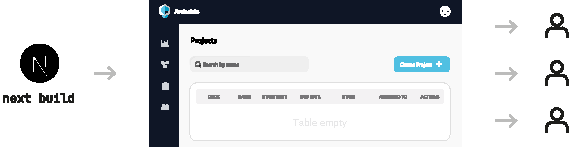
\includegraphics[width=0.7\textwidth]{img/rendering/static_generation.pdf} 
        \caption{Static Generation}
    \end{figure}
    
    
    \item \textbf{Server-side Rendering (SSR o Dynamic Rendering)}: il rendering lato server consente di generare dinamicamente il codice HTML per ogni pagina al momento della richiesta. Questo approccio è cruciale per le pagine che richiedono dati in tempo reale o informazioni che cambiano frequentemente. Con il Server-Side Rendering, ogni volta che un utente richiede una pagina, il server elabora le informazioni necessarie e genera il codice HTML. Una volta completato il rendering, l'HTML viene inviato al browser, assicurando che l'utente riceva immediatamente una pagina completamente renderizzata e aggiornata.
     \begin{figure}[H]
        \centering
        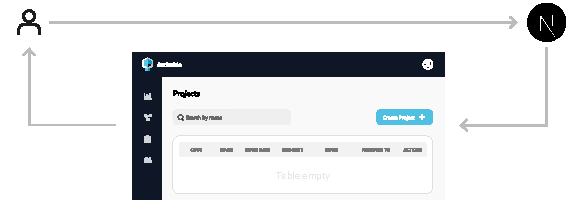
\includegraphics[width=0.7\textwidth]{img/rendering/server_side_rendering.pdf} 
        \caption{Server-side Rendering}
    \end{figure}
\end{itemize}

\noindent Come già descritto in precedenza, quando una pagina web è generata attraverso il rendering lato server, il server invia al browser un documento HTML già pronto, completo di contenuto e struttura. Tuttavia, affinché l'applicazione diventi interattiva e possa rispondere agli eventi (come click, input dell'utente, ecc.), è necessario che il codice JavaScript venga caricato e eseguito nel browser. 

\noindent Dunque, una volta che il codice JavaScript è disponibile, viene eseguito l'\texttt{hydration}, ossia un processo che comporta l'associazione dei gestori di eventi e l'attivazione della logica dei componenti, trasformando l'HTML statico in un'applicazione interattiva.

\begin{figure}[H]
    \centering
    \begin{subfigure}[b]{0.46\textwidth}
        \centering
        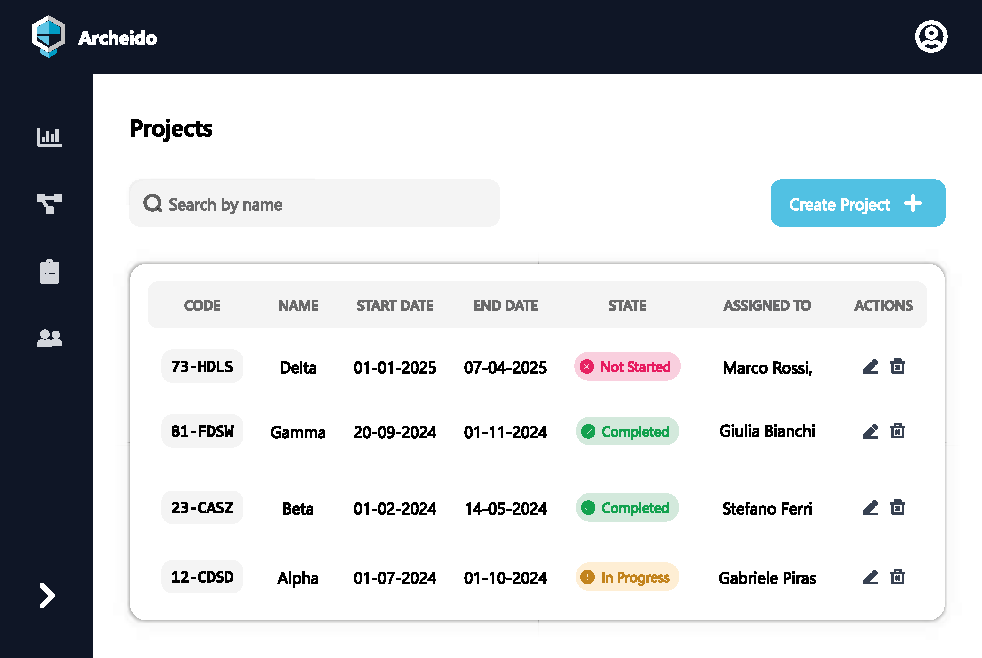
\includegraphics[width=\textwidth]{img/hydration/hydration1.pdf}
        \caption{\textbf{JavaScript non ancora caricato}: facendo clic sul pulsante di eliminazione di un progetto, non si verifica alcuna azione.}
        \label{fig:img1}
    \end{subfigure}
    \hfill
    \begin{subfigure}[b]{0.46\textwidth}
        \centering
        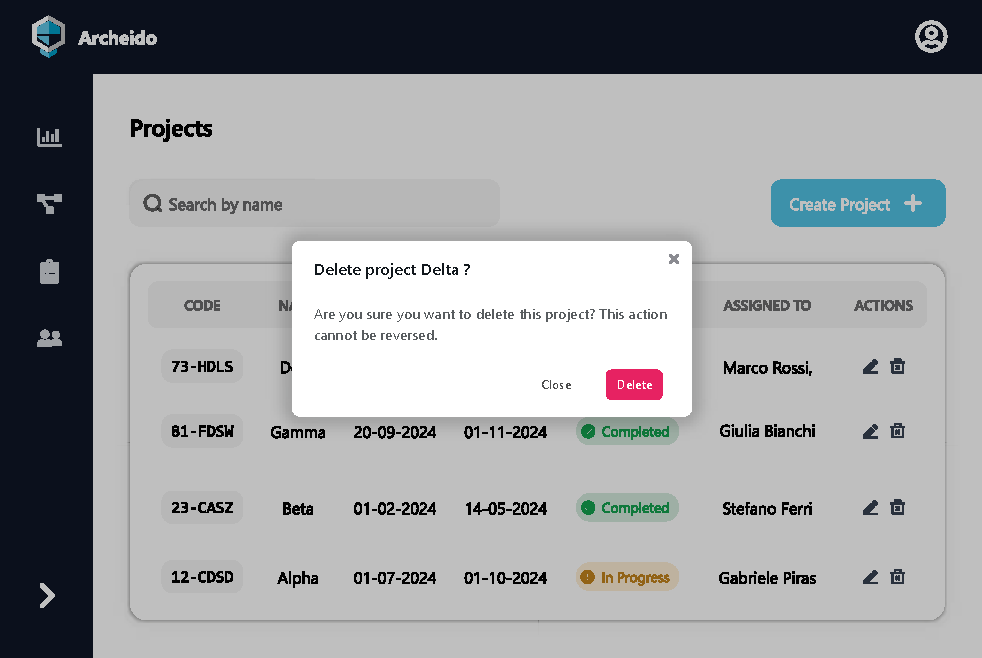
\includegraphics[width=\textwidth]{img/hydration/hydration2.pdf}
        \caption{\textbf{JavaScript caricato}: facendo clic sul pulsante di eliminazione di un progetto, si apre una finestra modale per confermare l'eliminazione.}
        \label{fig:img2}
    \end{subfigure}
    \caption{Prima e dopo l'hydration}
    \label{fig:two_images}
\end{figure}

\label{sec:hydration_error}
\noindent Sebbene l'hydration offra notevoli vantaggi in termini di prestazioni e SEO, durante la realizzazione di questo progetto si sono verificati diversi errori dovuti ad esso, evidenziati specialmente durante la fase di testing. Questi problemi erano principalmente dovuti a incongruenze tra l'HTML generato dal server e quello che il client si aspettava dopo l'esecuzione del codice JavaScript. In particolare, un componente utilizzava dati che cambiavano frequentemente, causando stati non sincronizzati tra server e client. La soluzione a questo problema è consistita nel trasferire la logica relativa agli stati problematici e non sincronizzati all'interno di un contesto, permettendo così di mantenere uno stato coerente tra server e client.

\subsection{App routing}
Il routing in React gestisce la navigazione tra diverse pagine o componenti all'interno di un'applicazione. Utilizza librerie come \texttt{React Router} per definire percorsi e associare URL specifici a componenti. Quando un utente naviga a un URL, React Router mostra il componente corrispondente senza ricaricare l'intera pagina, permettendo un'esperienza utente fluida e dinamica. In Next.js, il sistema di routing è reso notevolmente più semplice e intuitivo, poiché si basa sulla \textbf{struttura del file system}. Le cartelle rappresentano i percorsi nell'applicazione web, e ogni cartella dedicata a una pagina deve contenere un file chiamato \texttt{page.tsx}\footnote{L'estensione è \texttt{.tsx} perché si sta usando TypeScript. Con JavaScript sarebbe \texttt{.jsx}.}, che ne include il contenuto. La cartella \texttt{app} funge da radice del progetto. Ad esempio, nel CRM è stata creata una cartella \texttt{projects}, al cui interno si trova il file \texttt{page.tsx}. In questo file, è stata definita ed esportata una funzione che restituisce un elemento TSX. Questo componente verrà visualizzato quando si visiterà il percorso \texttt{./projects} nella pagina web.

\begin{figure}[H]
    \centering
    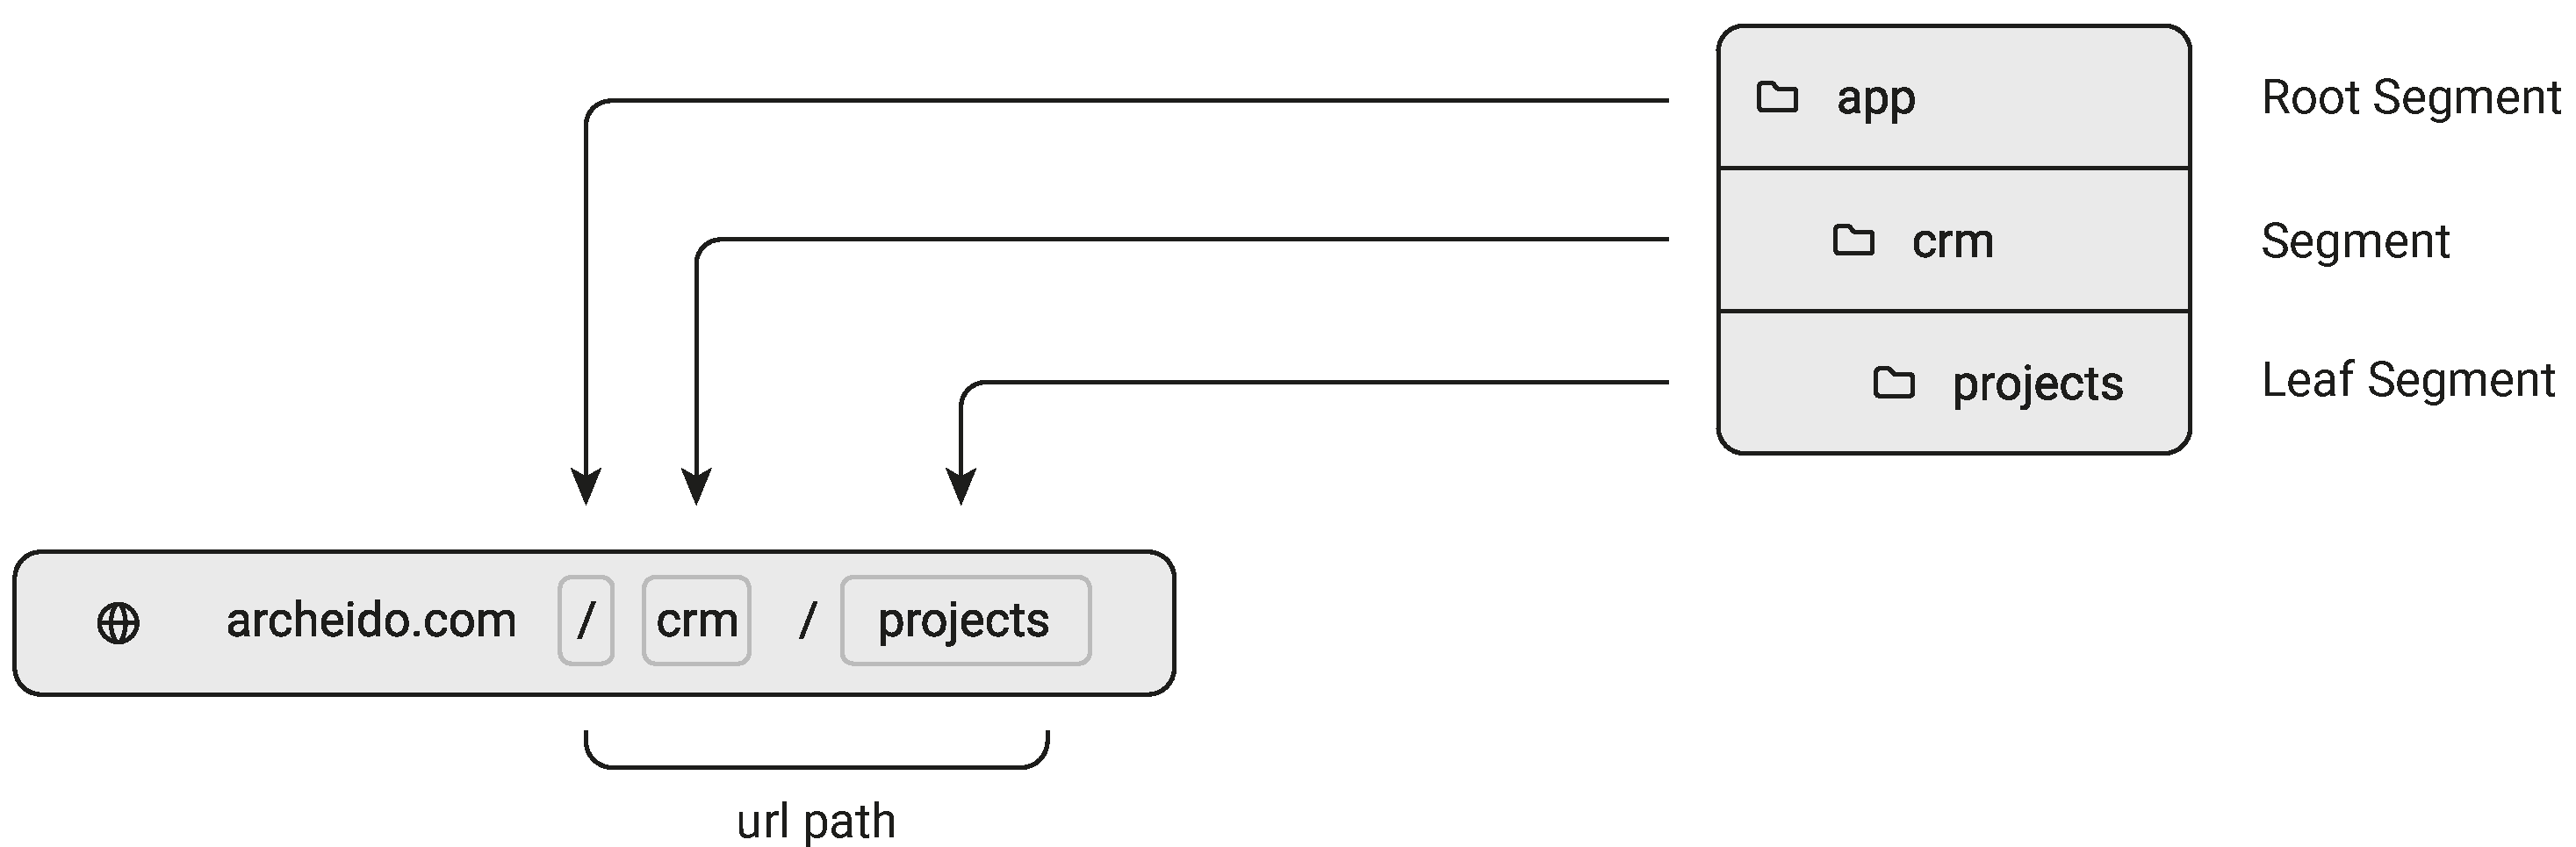
\includegraphics[width=0.9\textwidth]{img/routing.pdf} 
    \caption{App routing \cite{nextjsdocs2024} di Next.js}
\end{figure}

\noindent La gestione del routing è stata implementata utilizzando un hook specifico chiamato \texttt{useRouter}. Questo hook, fornito da Next.js, permette di accedere al router e gestire la navigazione all'interno dell'applicazione. Per utilizzarlo, è sufficiente importarlo con la seguente istruzione:

\begin{center}
    \texttt{import \{ useRouter \} from 'next/router';}
\end{center}

\noindent Dopodiché, può essere dichiarato all'interno del componente con la seguente sintassi:

\begin{center}
    \texttt{const router = useRouter();}
\end{center}

\noindent Utilizzando la costante \texttt{router}, è possibile accedere facilmente a numerose informazioni e funzionalità legate alla navigazione. In particolare, si possono ottenere:

\begin{itemize} 
    \item Il \textbf{percorso attuale}: con \texttt{router.pathname}, che restituisce il percorso della route corrente senza includere i parametri della query. Questo può essere utile per sapere quale pagina è attualmente visualizzata e per applicare logiche condizionali basate sulla posizione dell'utente nell'applicazione;
    \item I \textbf{parametri della query string}: tramite \texttt{router.query}, che fornisce un oggetto contenente i parametri della query presenti nell'URL. Questa funzionalità è utile per leggere dati dinamici dalla route, come identificatori o filtri passati tramite l'URL;
    \item \textbf{Funzioni per navigare a nuove route e gestione della cronologia del browser}: ad esempio, \texttt{router.push()} consente di navigare verso un nuovo percorso specificato, permettendo reindirizzamenti programmatici all'interno dell'applicazione. Un'alternativa è \texttt{router.replace()}, che, a differenza di \texttt{push()}, sostituisce la voce corrente nella cronologia del browser, evitando di aggiungerene una nuova. Infine, \texttt{router.back()} offre la possibilità di tornare alla pagina precedente, simulando il comportamento del pulsante ``indietro" del browser.
\end{itemize}

\noindent Nel contesto della web app sviluppata, questo hook è stato usato molte volte nel seguente modo:

\begin{lstlisting}[caption=\texttt{useRouter} per la navigazione tra URL]
import { useRouter } from 'next/router';
const MyComponent = () => {
    const router = useRouter();
    const handleNavigation = () => {
        router.push('/new-page'); // Reindirizza a "/new-page"
    };
    return (
        <div>
            <p>Current path: {router.pathname}</p>
            <p>Query params: {router.query}</p>
            <button onClick={handleNavigation}>Go to new page</button>
        </div>
    );
};
\end{lstlisting}

\noindent Un altro aspetto chiave di Next.js è la possibilità di implementare facilmente il \textbf{routing dinamico}. Questa funzionalità è stata adottata nella pagina \texttt{./projects} dove, selezionando un progetto, si accede ai relativi dettagli, con un reindirizzamento a una pagina avente un URL del tipo \texttt{/projects/ID\_PROGETTO}. Naturalmente, ogni progetto ha un URL univoco, il che rende funzionale la navigazione e il caricamento delle informazioni specifiche relative a ciascun progetto. Per ottenere ciò, all'interno della cartella \texttt{/projects} è stata creata un'ulteriore cartella denominata \texttt{[projectId]}. Questa convenzione di denominazione, utilizzando le parentesi quadre, indica a Next.js che il file al suo interno rappresenta una \textit{route dinamica}. All'interno di questa cartella, è presente un file chiamato \texttt{page.tsx}, che funge da componente per la pagina dei dettagli del progetto.

\begin{lstlisting}[caption=Routing dinamico con Next.js]
const page = ({ params }: { params: { projectId: string } }) => {
  const [selectedProject, setSelectedProject] = useState<Project>({});
  
  useEffect(() => {
    getProject(params.projectId).then((selectedProject: any) => {
      setSelectedProject(selectedProject as Project);
    });
  }, []);

  return <div>Selected project: {params.slug}</div>
};
\end{lstlisting}

\noindent Quando il componente viene montato, il codice esegue un effetto collaterale utilizzando l'hook \texttt{useEffect}. Questo effetto invoca la funzione \texttt{getProject}, passando il \texttt{projectId} come argomento per recuperare i dettagli del progetto corrispondente. Una volta ottenuto il progetto, lo stato \texttt{selectedProject} viene aggiornato con i dati ricevuti. Infine, il componente restituisce un elemento \texttt{<div>} che visualizza un messaggio con il slug presente in \texttt{params}. Questo messaggio indica quale progetto è stato selezionato. 

\section{Next UI e Tailwind CSS}

\subsection{Next UI}
In questo lavoro si è deciso di utilizzare Next UI \cite{nextui2024}, una libreria di componenti UI progettata specificamente per Next.js. Essa offre una serie di componenti predefiniti (come bottoni, calendari, modali, cards, chips, etc.) e stilizzati che semplificano la creazione di interfacce utente. Inoltre, è possibile importare solo i componenti necessari e non tutta la suite, riducendo il peso complessivo dell'applicazione. Ad esempio, se si volesse importare un componente relativo ad un calendario, sarebbe sufficiente scrivere il relativo codice:

\begin{figure}[H]
    \centering
    \begin{minipage}{0.6\textwidth}
        \begin{lstlisting}[caption=Uso di un componente NextUI]
import {Calendar} from "@nextui-org/react";

const date = parseDate("2020-02-03");
    
export default function App() {
    return (
        <Calendar 
            aria-label="Date" 
            defaultValue={date} 
        /> 
    );
}
        \end{lstlisting}
    \end{minipage}%
    \hfill
    \begin{minipage}{0.35\textwidth}
        \centering
        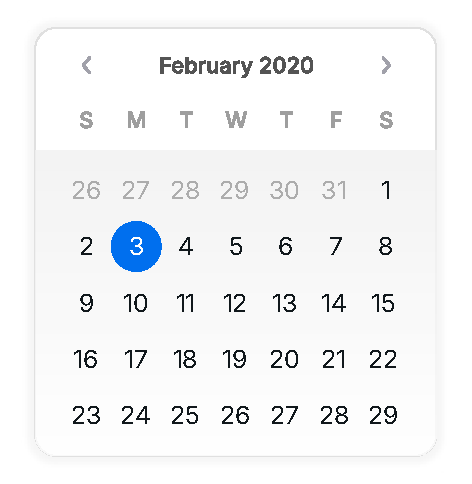
\includegraphics[width=\textwidth]{img/calendar.pdf}
        \caption{Calendario di NextUI}
    \end{minipage}
\end{figure}

\subsection{Tailwind CSS}
\noindent Un'altra libreria utilizzata per la progettazione del CRM di Archeido è Tailwind CSS: un framework CSS \textit{utility-first} che permette agli sviluppatori di creare interfacce utente in modo rapido e flessibile. Il termine \textit{utility-first} si riferisce a un approccio relativo alla progettazione delle interfacce utente che prevede l'uso di classi CSS predefinite per applicare gli stili direttamente agli elementi HTML, anziché creare classi personalizzate o definire stili specifici per i componenti. Un esempio è il seguente:

\begin{lstlisting}[caption=Parte del file \texttt{app.tsx} del CRM]
<main className = "flex flex-col h-screen">
    <NavBar className = "w-screen" signOut={signOut} />
    <div className = "flex flex-row h-full">
        <div className = "col-auto">
            <SideBar />
        </div>
        <div className = "col-auto p-8 grow">{children}</div>
    </div>
</main> 
\end{lstlisting}

\noindent Questo codice rappresenta la struttura di un componente React che definisce la disposizione generale delle pagine del progetto. L'elemento \texttt{<main>} ha una classe che lo rende un contenitore flessibile e verticale, con un'altezza che occupa l'intero schermo. All'interno di questo contenitore, è presente una barra di navigazione \texttt{<NavBar>} che si estende per tutta la larghezza della pagina e riceve una proprietà \texttt{signOut} per la gestione del logout. Sotto la barra di navigazione, vi è un contenitore diviso orizzontalmente in due sezioni. La prima sezione contiene una barra laterale \texttt{<SideBar>} che occupa spazio in base al suo contenuto, mentre la seconda sezione si estende e cresce per occupare il resto dello spazio disponibile. Quest'ultima include un'area di contenuto, rappresentata da \texttt{{children}}, che è un segnaposto per i contenuti passati come figli al componente principale

\begin{figure}[H]
    \centering
    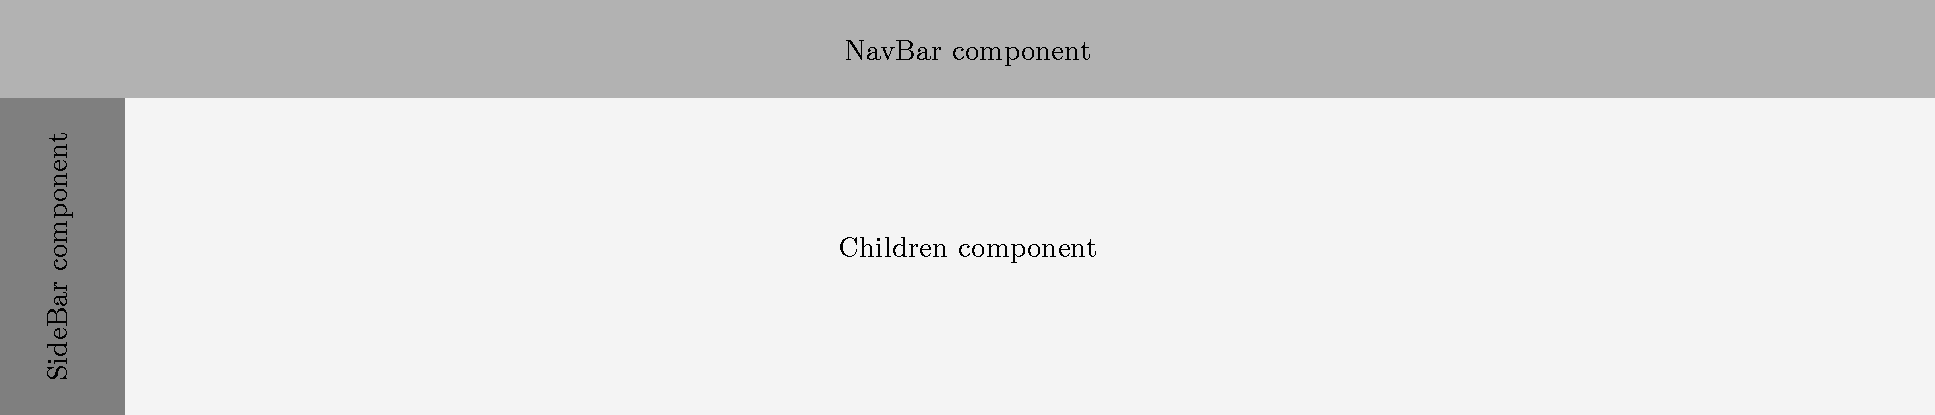
\includegraphics[width=1\textwidth]{img/layout.pdf} 
    \caption{Layout generico delle pagine, ottenuto utilizzando Tailwind CSS}
\end{figure}


\section{AWS: Amazon Web Service}
Nel contesto del CRM per la gestione dei progetti, è stato scelto Amazon Web Services (AWS) come piattaforma di hosting e gestione delle funzionalità del sistema. AWS offre una vasta gamma di servizi cloud che si integrano in modo efficiente per garantire scalabilità, sicurezza e affidabilità.

\noindent Per il deployment e la gestione del front-end del CRM, è stato impiegato \textbf{AWS Amplify}, un servizio che permette di ospitare applicazioni web con un'integrazione continua (CI/CD). Amplify è stato inizialmente collegato al repository \textbf{BitBucket}, il quale contiene il codice sorgente del progetto. Ogni volta che vengono effettuate modifiche al codice nel repository, Amplify esegue automaticamente un nuovo deployment.

\noindent Per la gestione dell'autenticazione degli utenti, è stato invece utilizzato \textbf{AWS Cognito}, il quale offre una gestione sicura delle credenziali, supportando funzionalità come la multi-factor authentication (MFA) e la rotazione automatica delle chiavi. Il sistema di login del CRM è progettato in modo tale da non permettere la registrazione autonoma degli utenti. Infatti, gli amministratori sono gli unici autorizzati a creare nuovi account e fornire le credenziali di accesso. Questo avviene direttamente dalla dashboard di Cognito, in quanto nel CRM non è stata sviluppata una funzionalità per rendere possibile l'invito di nuovi utenti, essendo uno scenario che trova impiego in pochi casi. Per implementare l'autenticazione, AWS mette a disposizione un componente \texttt{Authenticator}, il quale prende la prop \texttt{hideSignUp}, che permette di nascondere l'opzione per la registrazione.

\begin{lstlisting}[caption=Parte del file \texttt{AuthenticatedLayout.tsx} del CRM]
const AuthenticatedLayout = ({ children }: any) => {
    return (
    <Authenticator hideSignUp components={components}>
        {(props) => <App {...props}>{children}</App>}
    </Authenticator>
    );
};
\end{lstlisting}

\begin{figure}[H]
    \centering
    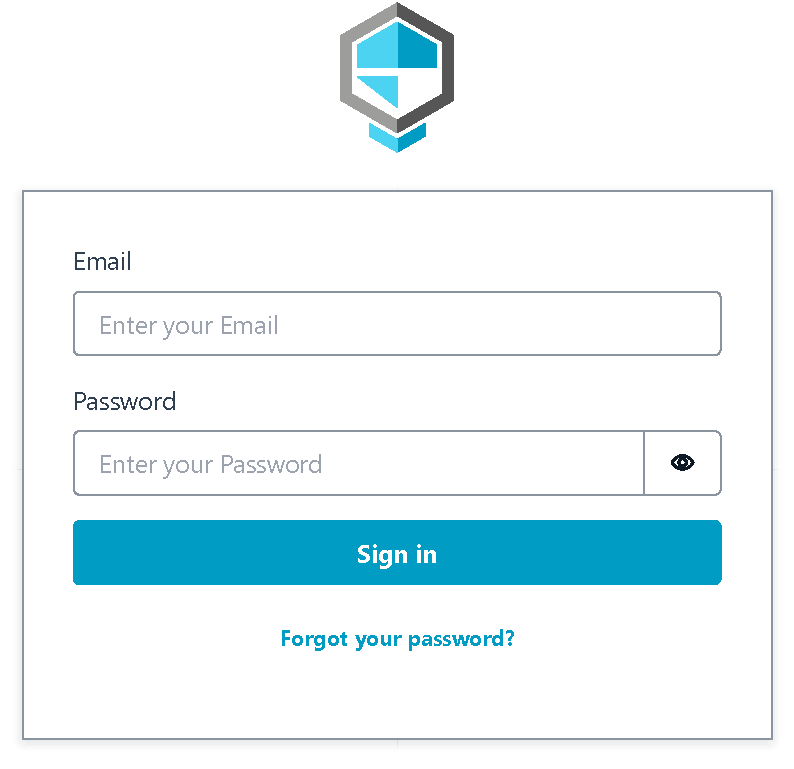
\includegraphics[width=0.5\textwidth]{img/login.pdf} 
    \caption{Pagina di login}
\end{figure}


% Capitolo 4
\chapter{Descrizione dei requisiti}

\section{Introduzione}
In questo capitolo si descriveranno i requisiti del sistema CRM per la gestione dei progetti, sviluppato durante il tirocinio. Verranno utilizzati diversi strumenti di modellazione per rappresentare i requisiti funzionali e non funzionali del sistema, tra cui diagrammi e pseudocodice per i casi più rilevanti.

\section{Definizione dei requisiti del sistema}
Il sistema CRM è stato progettato per supportare la gestione di progetti aziendali, offrendo funzionalità che spaziano dalla creazione e monitoraggio dei progetti, alla gestione degli utenti. I principali requisiti funzionali delineati durante la fase di raccolta dei requisiti includono:

\begin{itemize}
    \item \textbf{Gestione utenti e ruoli}: gli utenti con ruolo \texttt{ADMIN} possono accedere e apportare modifiche a tutte le sezioni della dashboard: è loro compito assegnare un progetto a uno o più project manager. Gli utenti con ruolo \texttt{PROJECT\_MANAGER} possono visionare, modificare e/o cancellare solo i progetti a cui sono stati assegnati da un utente con ruolo \texttt{ADMIN}. Inoltre, la sezione utenti, disponibile al link \texttt{./users}, è visibile solo ad utenti con ruolo di amministratore.
    \item \textbf{Accesso riservato ad utenti invitati}: un nuovo utente che desidera utilizzare il CRM deve ricevere un invito via e-mail contenente una password temporanea, inviato da un amministratore. Al primo accesso, l'utente sarà obbligato a cambiare la password temporanea.
    \item \textbf{Creazione di un progetto}: l'utente può creare un progetto, specificando dettagli come \texttt{codice}, \texttt{nome}, \texttt{data\_di\_inizio}, \texttt{data\_di\_fine}, \texttt{stato} (il quale può assumere i valori di \texttt{non\_iniziato}, \texttt{in\_corso} o \texttt{completato}).
    \item \textbf{Modifica di un progetto}: l'utente può modificare un progetto esistente, cambiandone i campi sopracitati.
    \item \textbf{Cancellazione di un progetto}: l'utente può cancellare un progetto. 
\end{itemize}

\subsection{Gestione dei ruoli degli utenti}
Per implementare le regole di visibilità in base ai ruoli degli utenti, è stato aggiunto un campo custom dalla dashboard di Cognito: tale campo è stato definito come \texttt{ROLE} e può assumere solo i due valori sopracitati. Un utente che accede al CRM, viene memorizzato in un Context \footnote{è uno strumento (un oggetto) che consente di condividere dati (come lo stato o le funzioni) tra componenti senza dover passare esplicitamente le props attraverso ogni livello dell'albero dei componenti. Ogni volta che un campo del contesto varia, la schermata viene ri-renderizzata.} globale, il quale ``wrappa" l'intera appllicazione. Tale contesto può essere poi ottenuto in ogni componente della web app. 

\noindent Un esempio di utilizzo si può trovare nel componente \texttt{SideBar}. Una sidebar è un pannello laterale in un'interfaccia utente che offre accesso rapido finalizzato alla navigazione. In questo caso, il contenuto della sidebar varia in base al ruolo dell'utente attualmente loggato: se l'utente è un admin, ha accesso a tutte le sezioni: Performance, Projects, Orders e Users. Al contrario, se l'utente è un project manager, la sezione Users non sarà visibile. Per gestire le sezioni visibili nella sidebar, si utilizza un array di oggetti, il quale contiene l'insieme di sezioni visibili dall'utente con meno permessi, quindi project manager. 

\begin{lstlisting}[caption=Campi default visibili nella sidebar]
const menusFields = [
    {
        title: "Performances",
        src: "performances",
        icon: <FaRegChartBar className = "scale-150" />,
        visibility: "ALL",
        gap: false
    },
    {
        title: "Projects",
        src: "projects",
        icon: <FaProjectDiagram className = "scale-150" />,
        visibility: "ALL",
        gap: false
    },
    {
        title: "Orders",
        src: "orders",
        icon: <FaClipboardList className = "scale-150" />,
        visibility: "ALL",
        gap: false
    },
];
\end{lstlisting}

\noindent Viene successivamente estratto il ruolo dell'utente loggato dal contesto dell'applicazione:

\begin{lstlisting}[caption=Parte del file \texttt{AuthenticatedLayout.tsx} del CRM]
const user = useContext(AuthContext);
const role = user["custom:role"];
\end{lstlisting}

\noindent In questo modo, la costante \texttt{role} contiene la stringa \texttt{"ADMIN"} o la stringa  \texttt{"PROJECT\_MANAGER"}. Tale valore, viene usato in seguito per decidere se mostrare o meno la sezione Orders:

\begin{lstlisting}[caption=Verifica ruolo]
role === "ADMIN" 
    ? [...Menus, {
        title: "Users",
        src: "users",
        icon: <FaUserFriends className = "scale-150" />,
        visibility: "ADMIN",
        gap: false
    }]
    : Menus;
\end{lstlisting}

\noindent Questo codice verifica se il ruolo dell'utente che ha effettuato il login è ``ADMIN". Se è così, crea una nuova lista \texttt{Menus} che include gli elementi esistenti, aggiungendo un nuovo oggetto per la voce di menu ``Users". Contrariamente, se l'utente non è un admin, la lista \texttt{Menus} rimane invariata. 

\noindent L'uso dell'operatore di spread \texttt{...Menus} garantisce che la lista originale non venga modificata, mantenendo l'approccio immutabile tipico della programmazione funzionale.

\subsection{Operazioni di CRUD}
Le operazioni CRUD sono le quattro azioni fondamentali per la gestione dei dati in un database: Create (creare nuovi dati), Read (leggere o visualizzare i dati), Update (aggiornare i dati esistenti) e Delete (eliminare i dati). Il CRM supporta tutte e quattro queste operazioni, implementate seguendo la guida \cite{awsamplifynextjs2024} sulla documentazione di Amplify. Innanzitutto è stato creato il \textbf{modello dati} realtivo ai progetti

\begin{lstlisting}[caption=Parte del file \texttt{amplify/data/resource.ts}]
const schema = a
.schema({
    Project: a.model({
        code: a.string(),
        name: a.string(),
        startdate: a.string(),
        enddate: a.string(),
        state: a.string(),
        assignedTo: a.string(),
    }),
})
\end{lstlisting}

\noindent Ogni volta che si definisce un modello con \texttt{a.model()}, vengono automaticamente create le seguenti risorse nel cloud:
\begin{itemize}
    \item Una tabella DynamoDB per memorizzare i record.
    \item API per query che permettono di creare, leggere (list/get), modificare ed eliminare i record.
    \item Campi \texttt{createdAt} e \texttt{updatedAt} per tracciare quando ogni record è stato creato o aggiornato.
    \item API in tempo reale per iscriversi agli eventi di creazione, aggiornamento ed eliminazione dei record.
\end{itemize}
\noindent Una volta completata questa operazione, è stata creata una cartella \texttt{api} nella root del progetto. Questa cartella ha lo scopo di raggruppare tutti i file relativi alle chiamate API ed è stata pensata per mantenere il progetto ben organizzato, estraendo tutte le funzioni che effettuano chiamate al database. Al suo interno, è stata generata un'altra cartella denominata \texttt{Project}, che a sua volta contiene il file \texttt{endpoints.ts}. Quest'ultimo file si occupa di definire ed esportare le funzioni relative alle operazioni CRUD.

\noindent Le prime funzioni definite per gestire le operazioni di CRUD sono \texttt{getProject} e \texttt{listProject}. La funzione \texttt{getProject} accetta come argomento un ID di tipo stringa, effettua una richiesta al database e restituisce l'oggetto \texttt{Project} corrispondente. La funzione \texttt{listProject}, invece, recupera e restituisce l'intera lista dei progetti presenti nel database.

\begin{lstlisting}[caption=funzione \texttt{getProject}]
const getProject = async (id: string) => {
    const { data: selectedProject }: Project = await client.models.Project.get({
        id
    });
    return selectedProject;
};
\end{lstlisting}

\begin{lstlisting}[caption=funzione \texttt{listProject}]
const listProject = async () => {
    const { data: projects } = await client.models.Projects.list();
    return projects;
};
\end{lstlisting}

\noindent Graficamente, le due funzioni menzionate sono responsabili dell'estrazione di tutti i dati necessari dal database per popolare la tabella presente all'URL \texttt{/projects}, mostrata nell'immagine sottostante.

\begin{figure}[H]
    \centering
    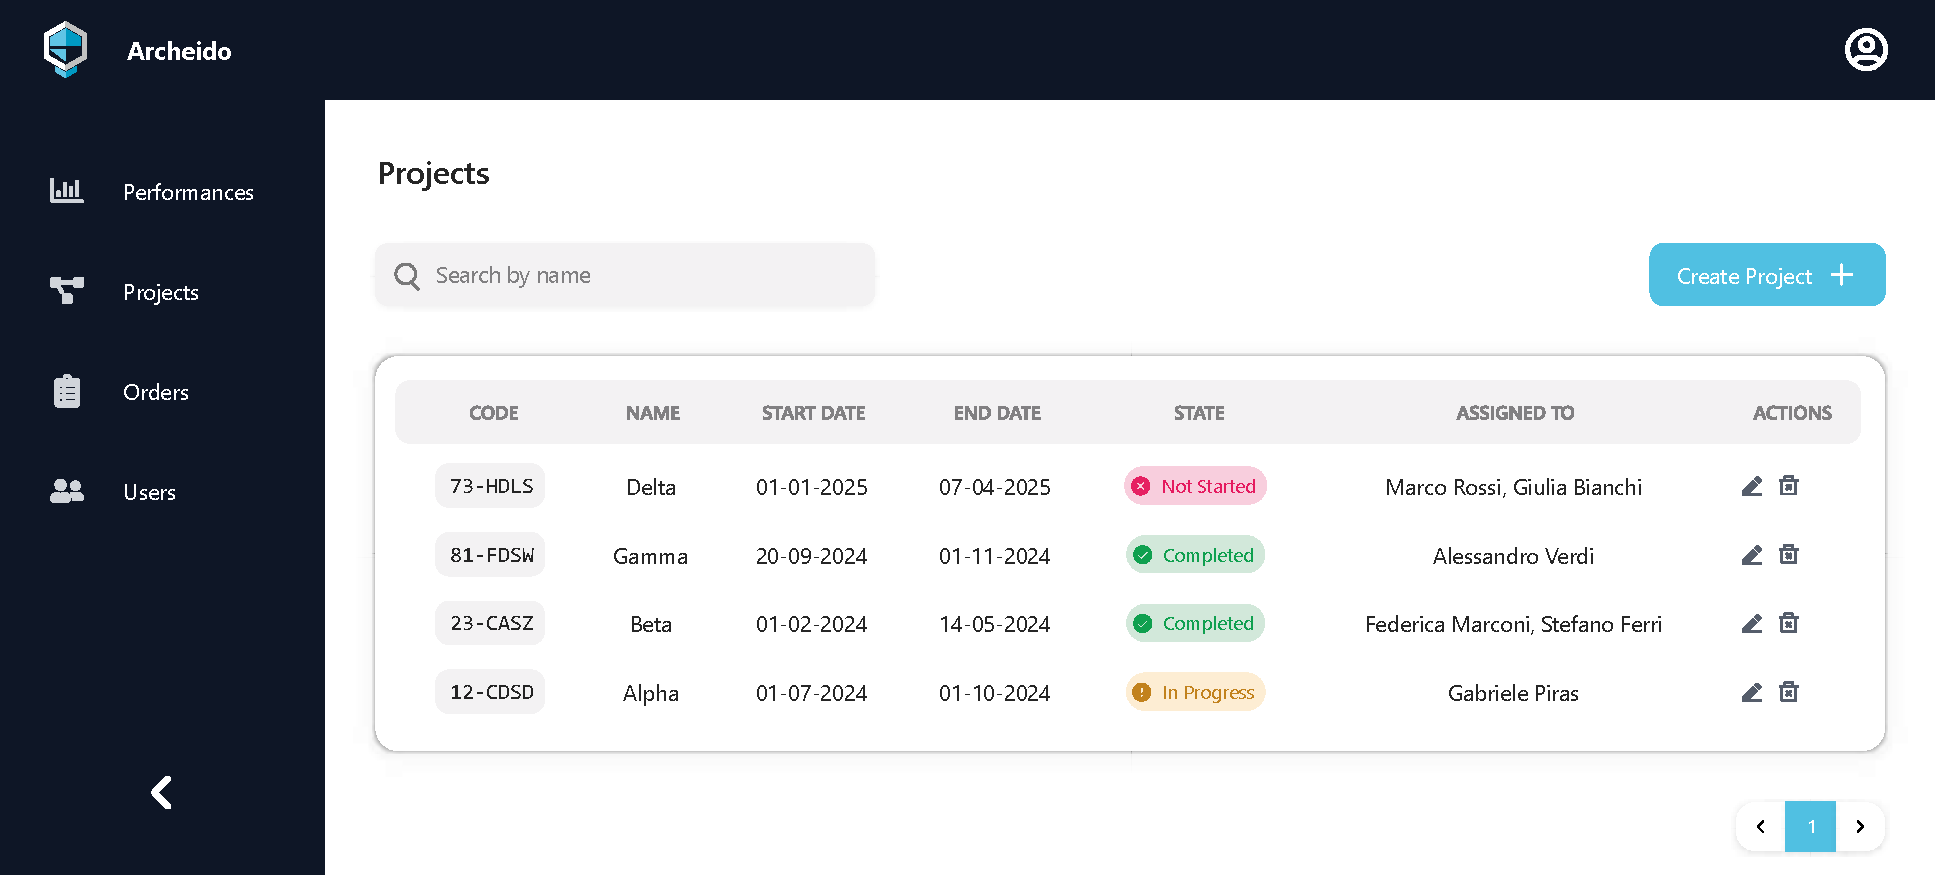
\includegraphics[width=0.8\textwidth]{img/interfacce/table_project.pdf} 
    \caption{Pagina dei progetti}
\end{figure}

\noindent A questo punto, se si clicca sul pulsante ``Create Project" viene caricato l'URL \texttt{./projects/create}, il quale visualizza un modulo vuoto per l'inserimento dei dati del progetto. Per la realizzazione e la gestione di questo modulo, è stata utilizzata la libreria \texttt{Formik}. Dopo aver compilato tutti i campi del modulo, premendo il pulsante ``Create" viene invocata la funzione \texttt{createProject}, che riceve come input l'oggetto \texttt{Project} generato tramite il riempimento dei campi e lo invia al database per la sua creazione.

\begin{lstlisting}[caption=funzione \texttt{createProject}]
const createProject = async (projectToCreate: Project) => {
    await client.models.Project.create(project);
};
\end{lstlisting}

\noindent La tabella dei progetti in \texttt{./projects} presenta una colonna denominata \texttt{ACTIONS}, in cui sono visibili due icone. Quando si preme l'icona a forma di cestino, si apre una modale di \textit{danger} che consente di confermare l'eliminazione del progetto. D'altro canto, se si seleziona l'icona a forma di matita, viene caricato l'URL della pagina del progetto con la seguente forma: \texttt{./projects/project\_id}. In quest'ultima è possibile effettuare modifiche o procedere all'eliminazione del progetto.

\noindent Per cancellare un progetto, si utilizza la funzione \texttt{deleteProject}, che richiede come argomento l'oggetto \texttt{Project} da eliminare, e tramite il suo ID, ne esegue la cancellazione:

\begin{lstlisting}[caption=funzione \texttt{deleteProject}]
const deleteProject = async (projectToDelete: Project) => {
    const { id } = projectToDelete;
    await client.models.Project.delete({ id });
};
\end{lstlisting}

\noindent L'aggiornamento di un progetto esistente viene eseguito mediante la funzione \texttt{updateProject}, che accetta come parametro un oggetto \texttt{Project} e aggiorna il database con i nuovi dati forniti:

\begin{lstlisting}[caption=funzione \texttt{updateProject}]
const updateProject = async (projectToUpdate: Project) => {
    await client.models.Project.update(projectToUpdate);
};
\end{lstlisting}

\begin{figure}[H]
    \centering
    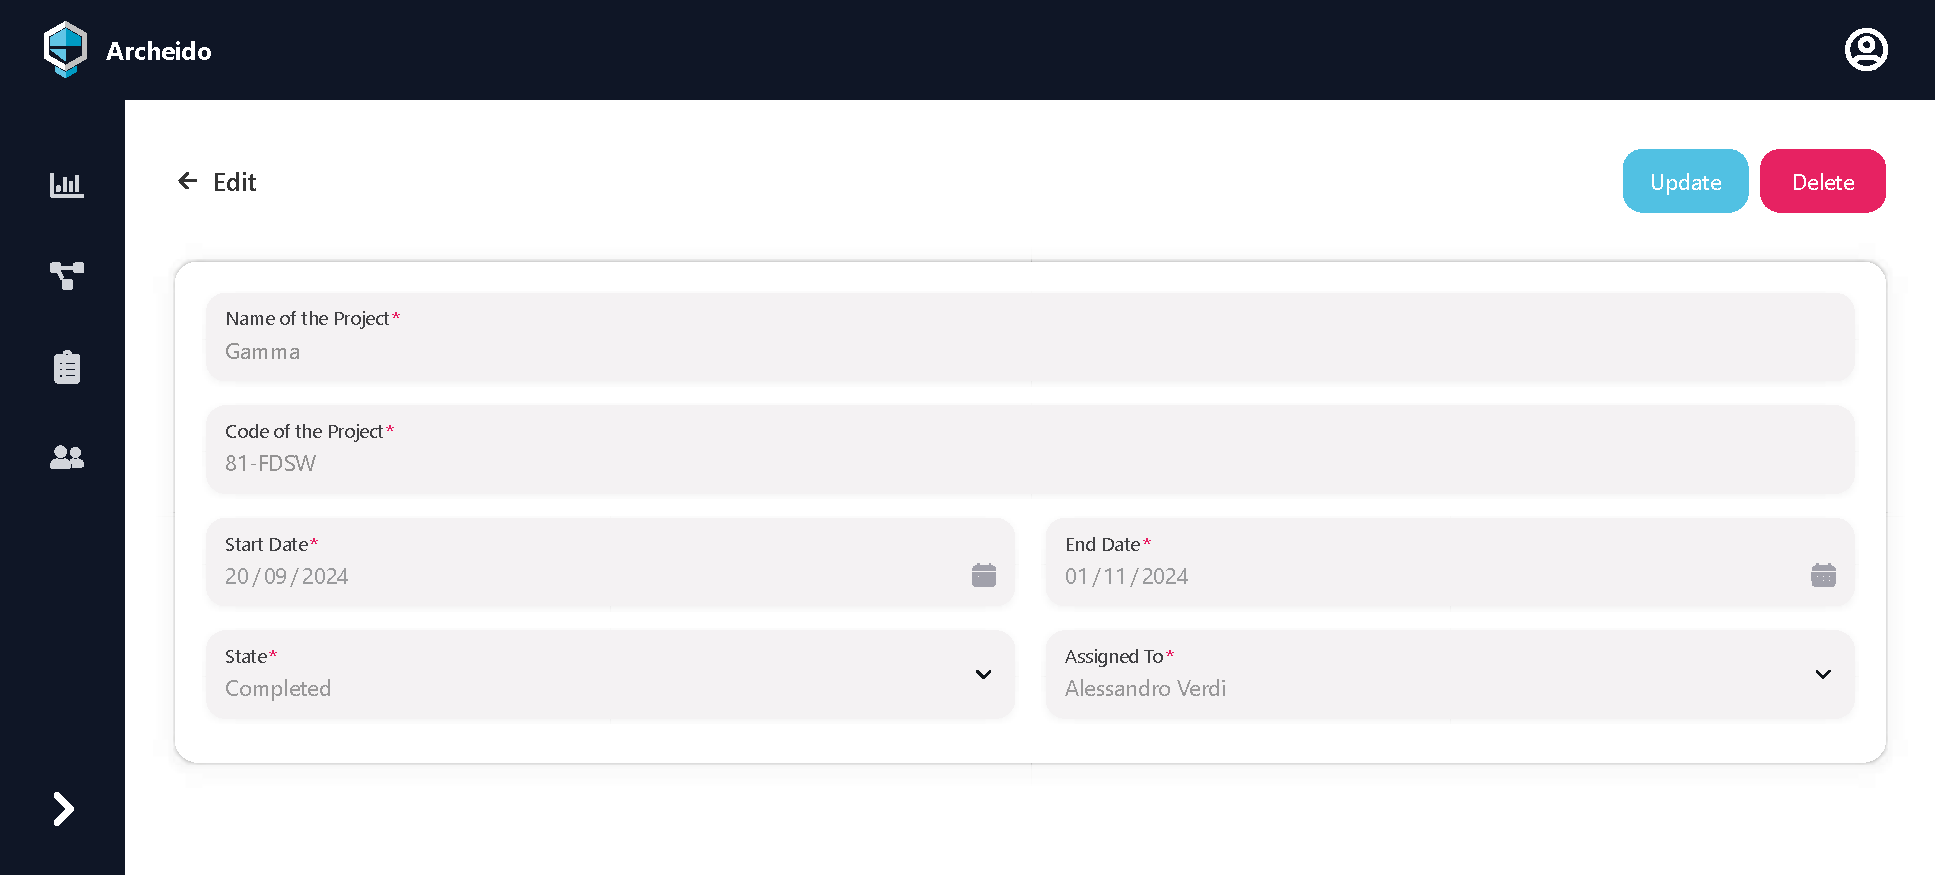
\includegraphics[width=0.8\textwidth]{img/interfacce/table_edit.pdf} 
    \caption{Pagina dei progetti}
\end{figure}

\section{Diagrammi}
\subsection{Diagramma dei casi d'uso (Use Case Diagram)}
Il diagramma nella figura mostra il sistema CRM con i diversi attori coinvolti, sia umani che esterni. Nello specifico:

\begin{itemize}
    \item gli \textbf{attori umani} includono ``User", ``Project Manager" e ``Admin" ;
    \item i \textbf{servizi esterni} sono ``AWS DynamoDB" e ``AWS Cognito".
\end{itemize}

\noindent Gli attori umani interagiscono con il sistema principalmente per la gestione dei progetti e degli utenti. Le operazioni di gestione dei progetti ne comprendono la creazione, lettura, aggiornamento e cancellazione, raggruppate sotto il caso d'uso generale ``Manage Projects". 

\noindent In modo simile (ma limitato agli attori Admin), la gestione degli utenti è modellata attraverso il caso d'uso ``Manage Users", che include funzionalità come invitare nuovi utenti, modificare i ruoli e cancellare utenti già registrati. 

\noindent Il processo di autenticazione è diviso in due casi d'uso principali: il ``First Login" per il primo accesso e ``Second + Login" per i successivi. Questi casi d'uso si estendono con la gestione degli errori e la verifica delle password. Inoltre, è presente un caso d'uso separato per il cambio della password, ``Change Password". Il sistema interagisce con ``AWS Cognito" per gestire l'autenticazione e con ``AWS DynamoDB" per eseguire operazioni sui dati dei progetti.

\begin{figure}[H]
    \centering
    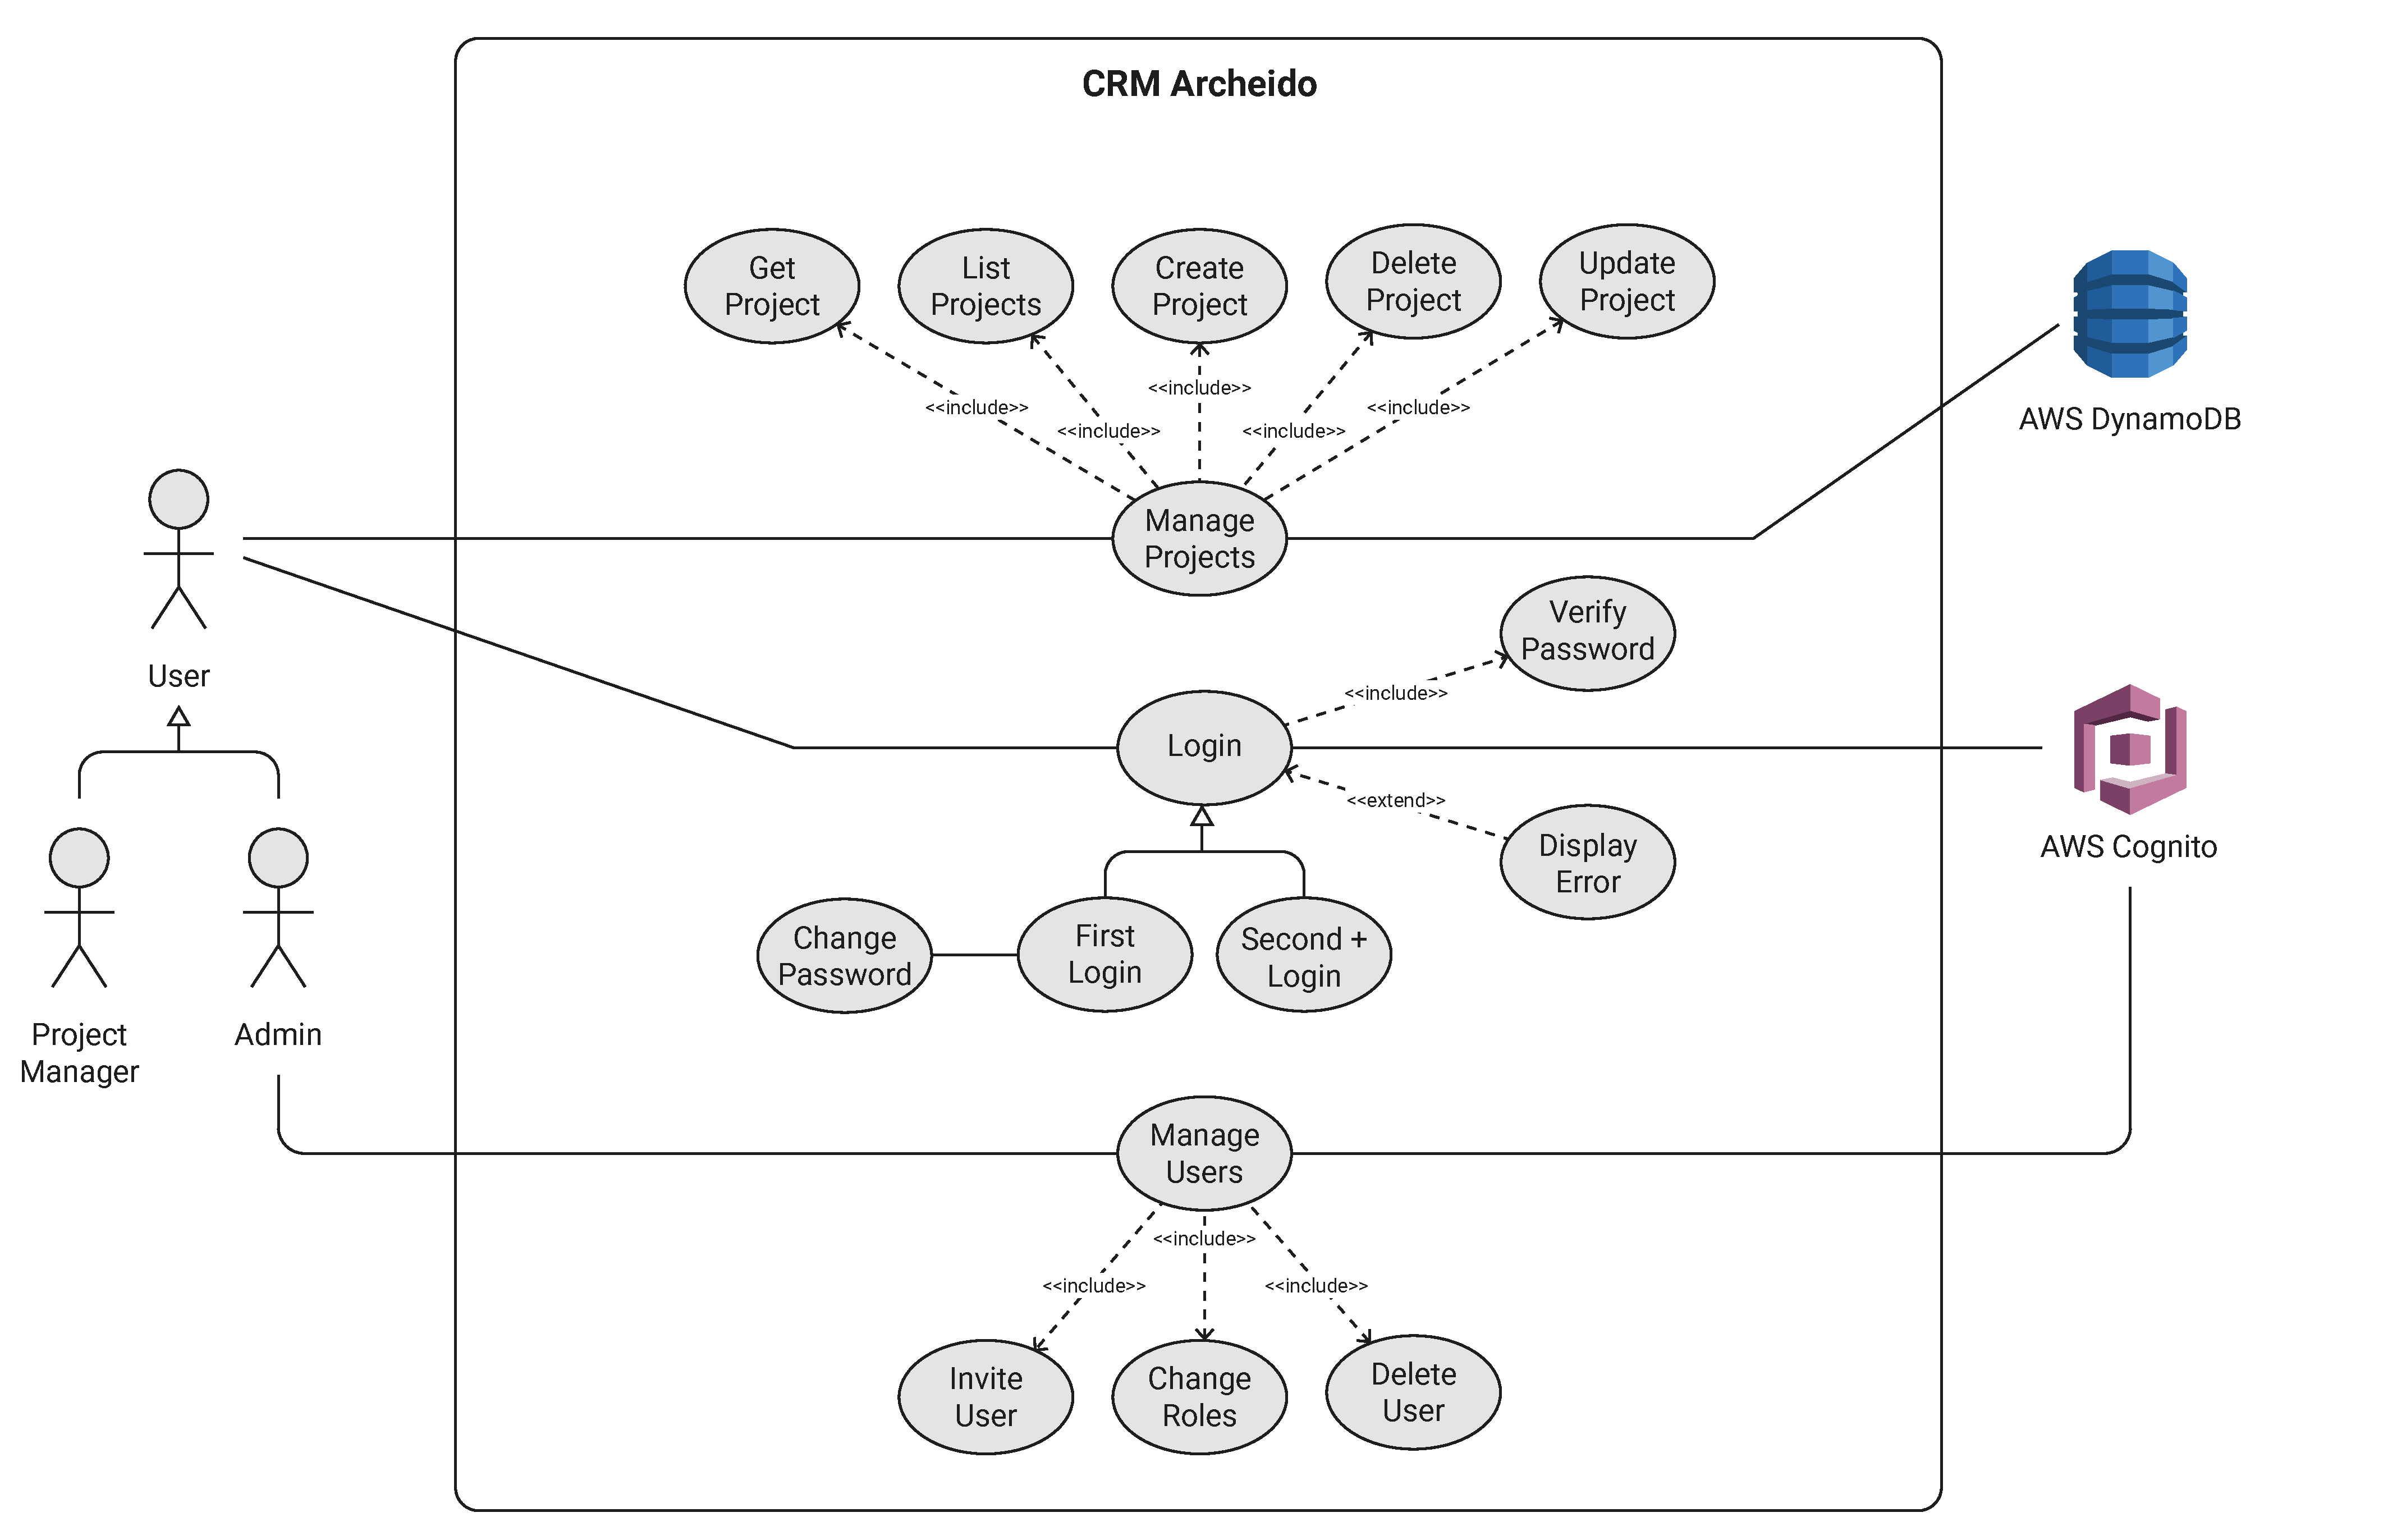
\includegraphics[width=1\textwidth]{img/diagrammi/use_case.pdf} 
    \caption{Use Case Diagram}
\end{figure}

\subsection{Sequence diagram}
Il diagramma di sequenza illustra le interazioni tra l'utente, il sistema di autenticazione Cognito, la dashboard del CRM e il database DynamoDB nella gestione dei progetti. Inizia con l'utente che inserisce le credenziali (e-mail e password) nella pagina di login, che inoltra i dati al pool di utenti Cognito per verificarne la validità. Se l'e-mail è presente e la password corretta, il client riceve una risposta di successo, confermando l'accesso; in caso contrario, viene visualizzato un messaggio di errore. Dopo un accesso riuscito, l'utente naviga alla pagina dei progetti (\texttt{/projects}), dove può visualizzare l'elenco di tutti i progetti disponibili. La dashboard del CRM richiede i dati al database DynamoDB tramite la funzione \texttt{listProject}, e, una volta ottenuta la risposta, i progetti vengono mostrati in una tabella. Quando l'utente desidera creare, modificare o eliminare un progetto, invia una richiesta tramite la dashboard. Per creare un nuovo progetto o cancellarne uno esistente, vengono invocate rispettivamente le funzioni \texttt{createProject} o \texttt{deleteProject}. Dopo l'esecuzione di queste operazioni, la dashboard aggiorna la lista dei progetti per mostrare i dati più recenti. Analogamente, se l'utente sceglie di aggiornare un progetto, viene invocata la funzione \texttt{updateProject} e i dati modificati vengono salvati nel database, con la lista dei progetti che si ricarica per riflettere le modifiche.

\begin{figure}[H]
    \centering
    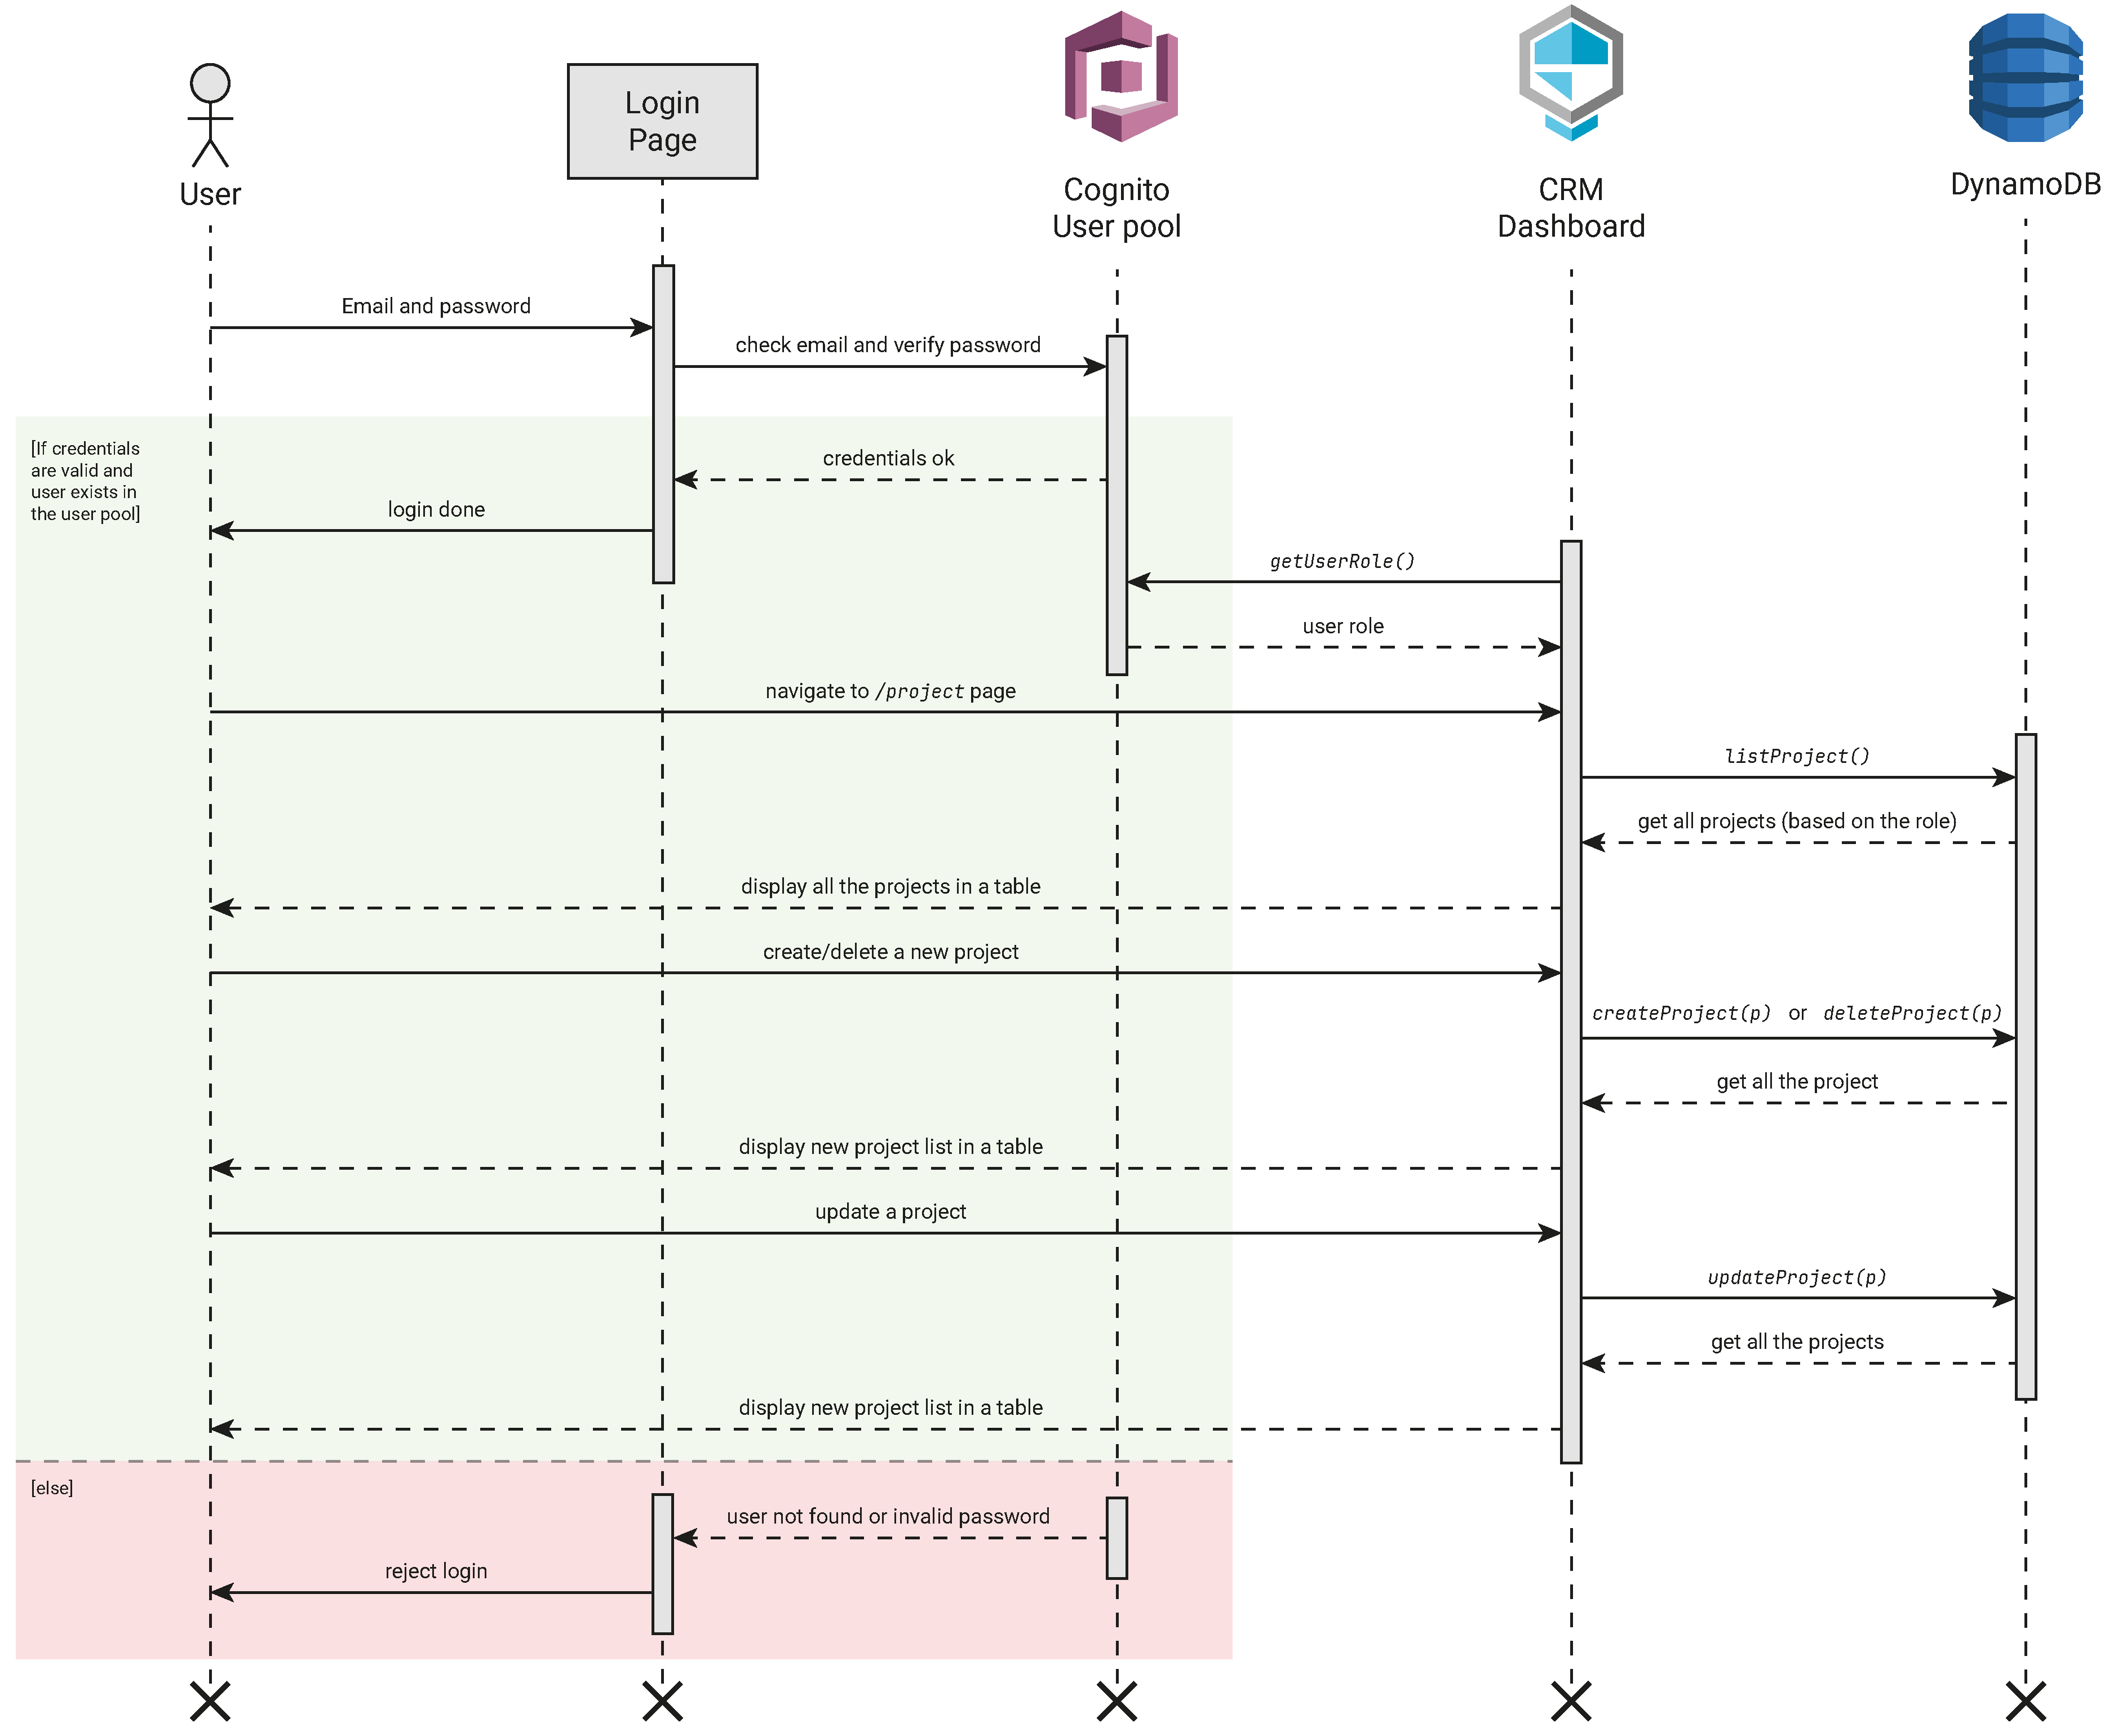
\includegraphics[width=1\textwidth]{img/diagrammi/sequence.pdf} 
    \caption{Sequence Diagram per il login e le operazioni CRUD sui progetti}
\end{figure}

% Capitolo 5
\chapter{Testing}
Le attività di testing si sono concentrate principalmente sulla verifica delle funzionalità principali dell'applicazione e sulla gestione degli accessi in base ai ruoli definiti, assicurando che ogni componente critico funzionasse correttamente e che l'assegnazione dei permessi rispettasse i criteri di sicurezza e operatività previsti. Tuttavia, il focus limitato a questi aspetti ha fatto emergere alcune lacune significative, in particolare per quanto riguarda l'accessibilità e l'inclusività dell'applicazione. Questi aspetti, sebbene non compromettano l'efficienza di base, indicano la necessità di una riflessione più approfondita e di un'analisi dettagliata, che verrà discussa in un secondo momento per evidenziare come migliorare l'esperienza complessiva degli utenti e garantire che l'applicazione sia fruibile da persone con esigenze diverse.

\section{Tipologie di test condotti}
Diversi tipi di test sono stati implementati per valutare le funzionalità, l'affidabilità e l'usabilità del sistema in modo progressivo e complementare. Dapprima, il testing unitario ha consentito la verifica puntuale delle singole funzioni e componenti del codice, garantendo la loro operatività in un contesto isolato. 

\noindent Successivamente, si è effetuato il testing di integrazione per analizzare la cooperazione tra i vari moduli, verificando l'interazione tra frontend e backend, nonché l'affidabilità delle chiamate ai servizi esterni come \texttt{DynamoDB} e \texttt{AWS Cognito}. 

\noindent Infine, il testing di accettazione ha coinvolto gli utenti finali, admin e project managers, fornendo un feedback per confermare che il sistema rispondesse alle esigenze aziendali e offrisse un'esperienza user-friendly.

\subsection{Testing unitario}
Il testing unitario è stato utilizzato per testare singole funzioni e componenti del sistema in un ambiente controllato, verificando che ciascun elemento funzionasse correttamente e in modo indipendente dagli altri. Ogni funzione, come quelle di creazione, lettura, aggiornamento e cancellazione dei progetti, è stata verificata in isolamento per assicurare che operasse come previsto e che le risposte fossero accurate e coerenti. In secondo luogo, il testing unitario ha reso più semplice il refactoring del codice, garantendo che i miglioramenti e le modifiche non compromettessero le funzionalità esistenti. La copertura dei test ha contribuito a costruire una base solida per i successivi livelli di test, come il testing di integrazione, dove si è verificata l'interazione tra più componenti del sistema per confermare che collaborassero senza problemi.

\subsection{Testing di integrazione}
Il testing di integrazione è stato condotto per verificare l'interazione tra diversi moduli del sistema, in particolare tra il frontend e il backend. Questo ha incluso test per garantire che le chiamate API al database \texttt{DynamoDB} restituissero i risultati attesi e che il sistema di autenticazione \texttt{AWS Cognito} funzionasse correttamente.

\subsection{Testing di accettazione}
Il testing di accettazione è stato realizzato coinvolgendo direttamente gli utenti finali nel processo per simulare scenari di utilizzo reale e ottenere un feedback autentico sull'efficacia del sistema. Gli utenti hanno avuto l'opportunità di testare le funzionalità principali del CRM, valutando sia la correttezza tecnica delle operazioni, sia la fluidità e l'intuitività dell'interfaccia. Durante queste sessioni, sono stati verificati aspetti come la facilità di navigazione, la chiarezza dei flussi di lavoro e i tempi di esecuzione delle varie operazioni. Inoltre, questo tipo di testing ha garantito che il CRM rispondesse pienamente ai requisiti aziendali, rispettando i requisiti funzionali, definiti nelle prime fasi del progetto, e di performance.

\section{Casi di test}
I casi di test sono stati progettati con l'obiettivo di coprire in modo completo e dettagliato tutte le funzionalità principali del sistema, oltre a garantire la conformità ai requisiti funzionali stabiliti durante la fase di pianificazione iniziale del progetto. Questi casi di test sono stati sviluppati per esplorare scenari reali di utilizzo in modo da assicurare la robustezza e l'affidabilità dell'applicazione. L'attenzione è stata rivolta a verificare che ogni aspetto del sistema rispondesse correttamente agli input previsti e non, mantenendo un comportamento coerente e sicuro.  Di seguito vengono riportati alcuni esempi significativi di casi di test implementati:

\subsection{Test di creazione progetto}
\begin{itemize}
    \item \textbf{Obiettivo}: verificare che un progetto possa essere creato con successo.
    \item \textbf{Passi}:
    \begin{enumerate}
        \item Accedere come utente con ruolo \texttt{ADMIN}.
        \item Navigare alla pagina di creazione del progetto.
        \item Compilare il modulo con dati validi.
        \item Cliccare sul pulsante ``Create".
    \end{enumerate}
    \item \textbf{Risultato Atteso}: il progetto viene creato correttamente e compare nel relativo elenco dei progetti. Inoltre, anche dopo il refresh della pagina o dopo aver effettuato il logout e successivamente il login, il progetto rimane visibile e preservato nella lista, confermando la persistenza dei dati.
\end{itemize}

\subsection{Test di cancellazione progetto attraverso la pagina dei progetti}
\begin{itemize}
    \item \textbf{Obiettivo}: Verificare che un progetto possa essere cancellato correttamente direttamente dall'elenco dei progetti, senza la necessità di accedere alla pagina di dettaglio del progetto stesso.
    \item \textbf{Passi}:
    \begin{enumerate}
        \item Accedere come utente con ruolo \texttt{ADMIN}.
        \item Navigare alla pagina contentete la tabella con l'elenco dei progetti.
        \item Selezionare un progetto esistente dall'elenco e, facendo clic sull'icona a forma di cestino nella colonna delle azioni, verificare che si apra una finestra modale di conferma per la cancellazione.
        \item Cliccare sul pulsante ``Delete" nella modale.
    \end{enumerate}
    \item \textbf{Risultato Atteso}: il progetto viene rimosso con successo dall'elenco dei progetti. Inoltre, anche dopo un refresh della pagina o dopo aver effettuato il logout e poi il login, il progetto non deve più comparire nella lista.
\end{itemize}

\subsection{Test di cancellazione progetto attraverso la pagina del dettaglio}
\begin{itemize}
    \item \textbf{Obiettivo}: verificare che un progetto possa essere cancellato correttamente dalla pagina del dettaglio di tale progetto.
    \item \textbf{Passi}:
    \begin{enumerate}
        \item Accedere al sistema con un account avente ruolo \texttt{ADMIN}.
        \item Navigare alla pagina contenente la tabella con l'elenco dei progetti.
        \item Selezionare il progetto che si desidera eliminare, cliccando sull'icona a forma di matita nella colonna delle azioni per accedere alla pagina di dettaglio.
        \item Attendere il caricamento della pagina e, una volta completato, premere il pulsante ``Delete". Assicurarsi che appaia una finestra modale di conferma per la cancellazione.
        \item Confermare l'azione cliccando nuovamente sul pulsante ``Delete" nella modale di conferma.
    \end{enumerate}
    \item \textbf{Risultato Atteso}: il progetto viene rimosso con successo dall'elenco. Inoltre, anche dopo un refresh della pagina o dopo aver effettuato il logout e poi il login, il progetto non deve più comparire nella lista.
\end{itemize}


\subsection{Test di modifica progetto}
\begin{itemize}
    \item \textbf{Obiettivo}: assicurarsi che un progetto esistente possa essere modificato.
    \item \textbf{Passi}:
    \begin{enumerate}
        \item Accedere come \texttt{PROJECT MANAGER}.
        \item Selezionare un progetto dall'elenco.
        \item Modificare i dettagli del progetto.
        \item Cliccare sul pulsante ``Update".
    \end{enumerate}
    \item \textbf{Risultato Atteso}: le modifiche vengono salvate con successo e visualizzate correttamente, assicurando che gli aggiornamenti siano immediatamente riflessi nell'interfaccia e persistano nel sistema.
\end{itemize}

\subsection{Test di accesso riservato}
\begin{itemize}
    \item \textbf{Obiettivo}: assicurarsi che solo gli utenti autorizzati possano accedere a determinate funzionalità del sistema, come la visualizzazione dell'icona relativa alla pagina ``Users" nella barra laterale della dashboard o la navigazione all'URL \texttt{/users}.
    \item \textbf{Passi}:
    \begin{enumerate}
        \item Accedere come utente con ruolo \texttt{PROJECT MANAGER}.
        \item Verificare la mancanza della  sezione ``Users" nella barra laterale.
        \item Tentare di accedere alla sezione ``Users", scrivendo forzatamente nella barra degli URL del browser l'URL \texttt{/users}.
    \end{enumerate}
    \item \textbf{Risultato Atteso}: l'accesso viene bloccato e l'utente visualizza un messaggio di errore che informa sull'assenza delle autorizzazioni necessarie per accedere alla sezione ``Users".
\end{itemize}

\section{Risultati}
Il processo di testing ha prodotto risultati complessivamente positivi. Durante le fasi di verifica, sono stati identificati e risolti diversi bug minori, prevalentemente associati all'interfaccia utente e alla gestione degli stati dell'applicazione. Relativamente a quest'ultimi, particolarmente significativo è stato il problema dell'hydration, una criticità emersa durante i test e dettagliatamente descritta nella sezione \ref{sec:hydration_error}. Questa problematica ha influito sul modo in cui i dati venivano sincronizzati tra il server e il client, causando alcune anomalie visive e interattive nell'interfaccia.

\noindent In aggiunta, grazie alle metodologie Agile, ogni ciclo di testing ha permesso di coinvolgere attivamente gli utenti finali del sistema, garantendo che le loro esigenze e aspettative venissero tempestivamente integrate nel processo di sviluppo. L'adozione di un approccio iterativo ha semplificato l'identificazione delle aree di miglioramento, consentendo di allineare il prodotto alle reali esigenze e desideri degli utenti finali. La continua iterazione e il monitoraggio delle prestazioni del software, hanno contribuito a mantenere un elevato standard di qualità, assicurando che l'applicazione rispondesse ai requisiti iniziali e fosse anche capace di adattarsi a esigenze future e feedback emersi durante le fasi di testing.

\noindent Infine, le prestazioni del sistema sono state valutate favorevolmente e le operazioni di CRUD hanno mostrato tempi di risposta rapidi e consistenti e il feedback degli utenti durante il testing di accettazione è stato positivo.

\section{Aspetti non testati e proposte di miglioramento}
Durante il processo di testing del sistema CRM sviluppato, l'attenzione si è focalizzata principalmente sulla verifica della corretta implementazione delle funzionalità principali e sulla gestione delle operazioni di accesso. Tuttavia, alcune aree critiche, come la sicurezza o l'accessibilità, non hanno ricevuto un'analisi dettagliata e approfondita. 

\subsection{Test di sicurezza}
Durante il processo di testing, poiché il CRM era destinato ad essere un progetto interno all'azienda, la sicurezza del sistema non è stata analizzata in modo approfondito, evidenziando così una significativa lacuna da considerare. La mancanza di test di sicurezza potrebbe esporre l'applicazione a rischi significativi, come furti di dati, compromissioni della privacy e danni reputazionali. Per affrontare queste preoccupazioni, è fondamentale implementare un programma di test di sicurezza che sia continuativo, in modo da rilevare e risolvere le vulnerabilità man mano che emergono. 

\subsection{Test di accessibilità}
In particolare, non sono stati condotti test specifici sulla navigazione tramite tastiera, un aspetto molto importante per garantire l'accessibilità agli utenti che, per ragioni di disabilità o preferenze personali, non utilizzano il mouse. Inoltre, non sono stati eseguiti test di compatibilità con screen reader. La mancanza di test in questo ambito potrebbe limitare l'uso del sistema a una parte significativa degli utenti, nello specifico non vedenti o ipovedenti, i quali si affidano a tecnologie assistive per interagire con le applicazioni web. 

\noindent Per migliorare l'accessibilità e garantire che il CRM sia inclusivo, si propone di implementare in futuro una serie di test dedicati alla navigazione tramite tastiera e alla compatibilità con i principali screen reader. Attraverso la scrittura di test mirati al garantire l'accessibilità della web app, è possibile garantire che il sistema non solo soddisfi i requisiti funzionali, ma anche i principi di inclusività, rendendo l'esperienza utente davvero completa e soddisfacente per tutte le tipologie di utenti.



% Capitolo 6
\chapter{Conclusioni}

\section{Obiettivi raggiunti}
Il sistema CRM per la gestione dei progetti sviluppato durante il tirocinio ha soddisfatto gli obiettivi prefissati, fornendo una soluzione completa e scalabile per la gestione di progetti e utenti all'interno di un'organizzazione. Il progetto ha permesso l'implementazione di funzionalità chiave, tra cui:
\begin{itemize}
    \item La gestione centralizzata di utenti e ruoli, con accessi e permessi controllati basati sui ruoli \texttt{ADMIN} e \texttt{PROJECT MANAGER}, per una maggiore sicurezza e personalizzazione dell'esperienza.
    \item La creazione, modifica e cancellazione di progetti, con tracciamento dello stato e assegnazione dei responsabili, rendendo agevole il monitoraggio e la gestione delle attività.
    \item L'uso di strumenti come \texttt{AWS Cognito} e \texttt{DynamoDB}, che hanno consentito la gestione degli utenti e delle operazioni CRUD, supportando le necessità di autenticazione e archiviazione dei dati.
\end{itemize}

\section{Lezioni apprese}
Lo sviluppo del sistema CRM ha fornito numerose lezioni preziose, specialmente nell'ambito dell'uso di tecnologie come JavaScript, TypeScript, React e Next.js. L'integrazione di queste tecnologie ha permesso di costruire un'applicazione robusta e reattiva, ma ha anche comportato alcune sfide tecniche significative. L'uso di React, ad esempio, ha facilitato la creazione di interfacce utente dinamiche e modulari, ma ha reso necessaria una gestione accurata dello stato e delle proprietà per evitare problemi di performance e di rendering. Allo stesso modo, l'adozione di TypeScript ha offerto vantaggi in termini di tipizzazione statica, contribuendo a prevenire errori durante lo sviluppo, ma ha richiesto un'attenzione particolare alla definizione delle interfacce e delle strutture dei dati.

\noindent Le sfide tecniche affrontate durante lo sviluppo hanno ulteriormente sottolineato l'importanza di una pianificazione adeguata e di valutazioni rigorose per garantire la scalabilità futura del sistema. Dedicar tempo all'inizio del processo per costruire fondamenta solide e scalabili si è dimostrato essenziale, evitando così l'implementazione affrettata di funzionalità che potrebbero portare a problemi di scarsa scalabilità in futuro. In questo contesto, Next.js ha rivelato il suo valore, facilitando la gestione del rendering lato server e ottimizzando le prestazioni complessive dell'applicazione.

\noindent Inoltre, l'adozione di metodologie Agile ha mostrato numerosi benefici al progetto. Grazie alla suddivisione del lavoro in iterazioni brevi e incrementali, si è reso possibile ricevere feedback continui e apportare modifiche rapide e ``leggere" in base alle esigenze emergenti. Inoltre, le retrospettive regolari hanno favorito un ambiente di apprendimento continuo, dove le sfide e le soluzioni trovate sono state condivise.

\noindent In conclusione, l'esperienza di sviluppo del sistema CRM non solo ha evidenziato l'importanza di una solida pianificazione e di una gestione attenta delle tecnologie utilizzate, ma ha anche dimostrato come le metodologie Agile possano facilitare un approccio flessibile e reattivo, fondamentale per il successo di progetti complessi. Questo ha portato a un prodotto finale funzionale, scalabile e in grado di rispondere in modo efficace alle esigenze dei suoi utenti.

\section{Possibili sviluppi futuri}
Il sistema CRM ha fornito solide fondamenta, tuttavia esistono ulteriori opportunità di miglioramento e crescita. Di seguito verranno delineate alcune di queste possibilità.

\subsection{Potenziamento della logica di gestione degli stati}
Al momento, tutti gli stati di questa applicazione vengono gestiti nei componenti stessi attraverso l'hook \texttt{useState}. Tuttavia, questa modalità di gestione presenta svantaggi significativi, specialmente in contesti complessi. Ciò include difficoltà nella gestione dello stato globale, che porta a eccessivo \textbf{prop drilling}\footnote{è il processo di passaggio di props attraverso diversi livelli di componenti in React, fino a raggiungere il componente che ne ha bisogno. Questo rende il codice meno leggibile e più difficile da gestire, specialmente in applicazioni complesse con molti livelli di nidificazione.}, e complicazioni nella tracciabilità degli stati con l'aumento della complessità dell'applicazione. La gestione isolata di ciascuno stato può causare problemi di aggiornamenti concorrenti e inconsistenze nel rendering. Inoltre, la mancanza di centralizzazione rende difficile avere una visione complessiva dello stato dell'applicazione e complica i test automatizzati. Per queste ragioni, uno sviluppo futuro per questo progetto potrebbe essere quello di implementare una nuova logica per la gestione e il mantenimento degli stati attraverso l'utilizzo di contesti, reducer e il dispatch di azioni. 

\noindent Per iniziare, si potrebbe creare una cartella denominata \texttt{Context} e spostare al suo interno le logiche esistenti relative al contesto globale (ad esempio reperire i dati dell'utente loggato). In aggiunta, si potrebbe realizzare file separati relativi ai contesti, come \texttt{Project.tsx} e \texttt{Users.tsx}, i quali ``wrapperebbero" l'intera applicazione garantendo che le strutture dati all'interno dei contesti specifici siano accessibili in modo globale. Ogni contesto dovrà includere una costante \texttt{initState}, che definirà i dati iniziali e la struttura del contesto stesso. In questo nuovo approccio, le modifiche di stato non avverranno più tramite l'hook \texttt{useState}, ma piuttosto attraverso il dispatch di un'azione, che modificherà lo stato del contesto. Ogni volta che ciò si verificherà, l'applicazione verrà renderizzata nuovamente, proprio come accade con \texttt{useState}. Sfruttando questa metodologia, si potrà beneficiare di una gestione centralizzata e scalabile degli stati, semplificando la condivisione dei dati tra i componenti. Inoltre, contribuirà a migliorare la modularità e la manutenzione del codice, consentendo l'integrazione di funzionalità come un indicatore di \texttt{loading} durante i cambiamenti di stato o di pagina.

\subsection{Analisi dei dati}
Si potrebbe implementare funzionalità di data analytics per generare report dettagliati sulle performance dei progetti. Queste funzionalità consentiranno di raccogliere e analizzare dati significativi riguardanti le tempistiche di completamento, l'utilizzo delle risorse (ad esempio il tempo totale speso su un certo progetto rispetto a quello stimato inizialmente) e la soddisfazione dei clienti. Queste analisi potrebbero essere integrate nella pagina \texttt{/performances}, già presente nella struttura del progetto. All'interno di questa pagina, dovrebbe essere possibile visualizzare report interattivi e grafici che riassumono le performance dei progetti nel tempo, facilitando l'accesso a informazioni chiave per i manager e i team di progetto.

\subsection{Sviluppo di test sulla sicurezza e sull'accessibilità}
Si propone di includere test mirati nei seguenti ambiti: innanzitutto, la navigazione tramite tastiera, tramite test automatizzati che verifichino la navigabilità dell'interfaccia, con particolare attenzione agli elementi interattivi come pulsanti, link e moduli di input. Un'altra proposta è l'implementazione di test di compatibilità con screen reader comuni per assicurare che i contenuti siano esposti in modo comprensibile e sequenziale e che l'esperienza utente sia coerente. Altri test utili includono il controllo del contrasto cromatico, per assicurarsi che le scelte di colore siano conformi agli standard WCAG 2.1\cite{wcag21}. Inoltre, un'analisi approfondita delle etichette e delle descrizioni alternative sarebbe fondamentale per garantire che ogni immagine o icona disponga di un testo alternativo adeguato. 

\noindent Si suggerisce inoltre di implementare test di sicurezza per identificare e mitigare vulnerabilità nel software. Questo include test di penetrazione per simulare attacchi esterni e valutare la robustezza dell'applicazione. È importante anche eseguire analisi di vulnerabilità per individuare potenziali punti deboli. Ulteriori test devono riguardare la gestione delle sessioni, per assicurare che i dati degli utenti siano protetti e che le sessioni scadano in modo appropriato.

\subsection{Implementazione della gestione utenti}
Attualmente, la pagina dedicata agli utenti in \texttt{/users} consente esclusivamente la visualizzazione degli utenti registrati, senza offrire la possibilità di invitare nuovi utenti o di modificare i loro attributi. Una possibile nuova funzionalità potrebbe prevedere l'integrazione di una gestione completa degli utenti direttamente all'interno della dashboard del CRM, centralizzando così tutte le operazioni in un'unica interfaccia anziché attraverso la dashboard di Cognito.


% Capitolo 7
\chapter{Ringraziamenti}
Grazie



%\appendix
%\part{Appendici}
%\chapter{Titolo della prima appendice}

%% Bibliografia
\bibliographystyle{plain_\languagename}
\bibliography{thud}
\end{document}